\chapter{实验图像的科学呈现}

细胞生物学专业的研究生小苏正在整理一篇关于小分子化合物高内涵表型筛选的论文。为了在补充材料中展示对照孔（DMSO 处理）人骨肉瘤细胞（U2OS）的细胞核与线粒体荧光染色质量，她从显微镜工作站拷出几张图，顺手拖进幻灯片软件里把偏暗的线粒体面板“调亮一点、拉高对比度”，截屏保存成图片后，又把截图上传到一个生成式图像工具，输入指令“去噪、变清晰、提升分辨率”。

组会上，导师没有评价画面好不好看，只问了三个问题：第一，未经改动的 16 位原始文件保存在哪里？第二，细胞核与线粒体通道各自映射的是哪一段原始灰度值，对照视野之间用的是不是同一套显示范围？第三，右下角那根标着“$20\ \mu\text{m}$”的比例尺，是根据哪个物镜和相机像素尺寸算出来的？小苏一个也答不上来：截图早已把 16 位数值压成了 8 位 RGB，幻灯片滑块没有留下任何数值记录，比例尺则是照着另一篇论文的图估算着画上去的。

实验图像与本书第 6 章的流程图、第 7 章的机制示意图有着本质区别：\textbf{实验图像是测量，不是插画。}在显微镜照片、扫描电子显微镜（SEM）图像、蛋白印迹（Western blot）或组织病理切片中，每一个像素的数值都对应探测器在特定空间位置接收到的光子数或电子数。面对这类证据图像，AI 工具只承担三项辅助工作：协助整理呈现计划、起草确定性的图像读取与排版脚本、对导出图做格式与色觉等技术检查；\textbf{AI 绝不触碰证据图像的任何像素值。}本章围绕多通道荧光显微图与植物叶片扫描电镜图两类公开原始图像，拆解从原始文件管理、显示映射、伪彩色选择、裁剪与比例尺校准，到期刊图像诚信规则与完整交付记录的全流程。

\section{原始图像是证据：数据、显示与导出}

在数字成像系统中，\textbf{原始数据、显示设置与导出图}是三件完全不同的事物。混淆这三者，是绝大多数实验图像失真与合规问题的起点。

当科研级相机（如 sCMOS 或 CCD）采集一幅荧光显微图像时，光电探测器将每个像素位置收集到的光子转化为电荷，再由模数转换器（ADC）量化为整数灰度值，通常按单通道 12 位（数值范围 $0\text{--}4095$）、14 位（$0\text{--}16383$）或 16 位（$0\text{--}65535$）保存在未压缩的 TIFF 或仪器原生格式（如 OME-TIFF、ND2、CZI、LIF）中。这个二维整数矩阵才是测量数据。

然而，普通的电脑显示器、网页和文档阅读器每个颜色通道只能显示 8 位灰度（$0\text{--}255$）。要把 16 位文件里的原始数值呈现在屏幕上，看图软件必须执行一步\textbf{显示映射（display mapping）}：选定一个下限值（黑点，$v_{\min}$）和一个上限值（白点，$v_{\max}$），把小于或等于 $v_{\min}$ 的像素显示为纯黑（$0$），把大于或等于 $v_{\max}$ 的像素显示为纯白（$255$），并把中间的数值按比例映射到 $0\text{--}255$ 之间。在线性映射下，任意像素原始数值 $I$ 对应的 8 位显示灰度 $I_{\text{disp}}$ 为：
\[
I_{\text{disp}} = \operatorname{clip}\!\left(\frac{I - v_{\min}}{v_{\max} - v_{\min}},\, 0,\, 1\right) \times 255
\]
只要不覆盖原始文件，改变黑点和白点只是换了一副观察数据的“窗口”，底层 TIFF 文件里的测量值并未改变；可一旦在软件里点击“另存为 8 位 JPEG/PNG”或直接截图，映射范围之外的数值就会被永久截断，12 位或 16 位的精细灰度级也会被不可逆地压缩为 256 个灰阶。

我们用 Broad 研究所公开生物图像基准库 BBBC022v1（Gustafsdottir 等，2013；Ljosa 等，2012；权利人 Anne Carpenter 声明按 CC0 1.0 献入公有领域）中的真实原始图像来演示这一区别。本章主材料取自该数据集第 20585 号微孔板的 A13 孔（DMSO 溶剂对照，元数据标记为 \texttt{mock}）第 1 视野（\texttt{s1}）与第 2 视野（\texttt{s2}），包含两个单通道文件：通道 \texttt{w1} 为 Hoechst 33342 染色的细胞核，通道 \texttt{w5} 为 MitoTracker Deep Red 染色的线粒体。每个文件均为 $696 \times 520$ 像素的 16 位灰度 TIFF，但采集相机的有效位深为 12 位（理论上限 $4095$）。

读取第 1 视野细胞核通道（\texttt{w1}）的原始矩阵可知，全图 $361,920$ 个像素的数值分布在 $121\text{--}1655$ 之间，均值为 $238.4$，第 $0.1\%$ 与第 $99.9\%$ 分位数分别为 $132$ 与 $1236$，没有任何像素达到相机上限 $4095$。图~\ref{fig:ch08-01} 展示了这一份 16 位原始矩阵在三种线性显示映射下的画面及对应的原始数值直方图。

\begin{figure}[htbp]\centering
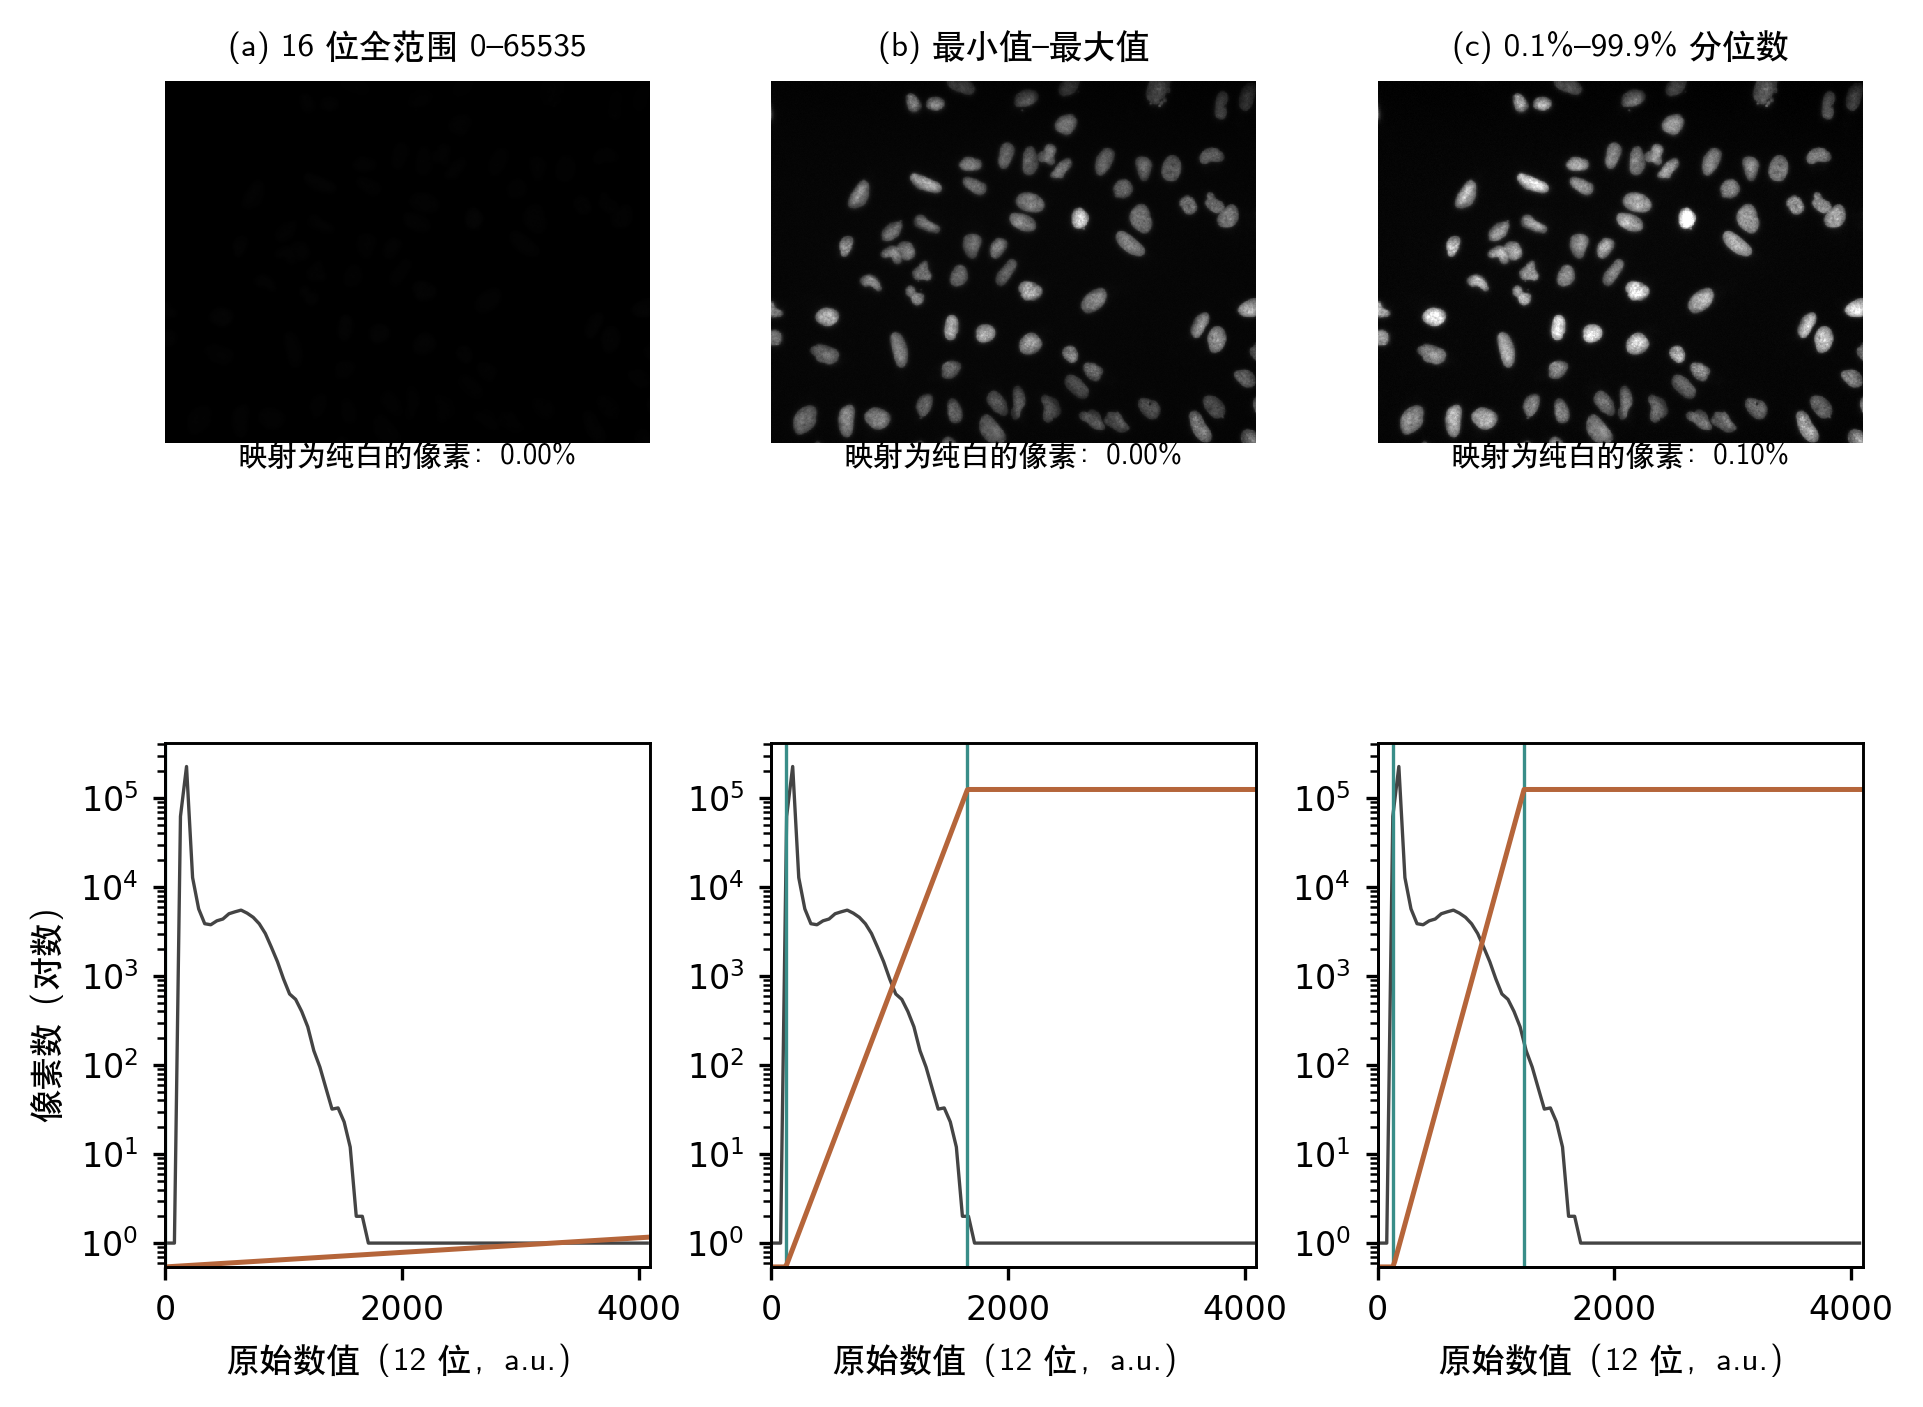
\includegraphics[width=0.88\linewidth]{figures/ch08/ch08-01-raw-display-mapping-zh.png}
\caption{同一幅 16 位荧光原图（BBBC022，Hoechst 通道）的三种线性显示。原始像素值在三列中完全相同，改变的只是显示映射：(a) 按 16 位全范围；(b) 按图像最小值至最大值；(c) 按 $0.1\%$ 与 $99.9\%$ 分位数，图中注明被映射为纯白的像素比例。下排为原始数值直方图与映射线。图像：BBBC022v1，CC0。}\label{fig:ch08-01}
\end{figure}

对照图~\ref{fig:ch08-01} 的三列，可以清楚看到显示映射如何改变画面外观：
\begin{itemize}
\item \textbf{列 (a)（按 16 位容器全范围 $0\text{--}65535$ 线性映射）：}许多操作系统的自带看图器在打开 16 位 TIFF 时，默认把 $0$ 当作黑点、$65535$ 当作白点。由于 12 位相机的读数不会超过 $4095$，且该视野细胞核的最高值仅为 $1655$，最亮的像素在映射后也只有 $1655 / 65535 \times 255 \approx 6.4$ 的灰度值。结果上排左图看起来几乎全黑（映射为纯白的像素为 $0.00\%$），下排直方图中的棕色映射直线紧贴在横轴底部。不少初学者看到这团漆黑，误以为拍摄失败，或者急忙用修图软件“拉亮并保存”，无意间毁掉了原件。
\item \textbf{列 (b)（按图像最小值至最大值 $121\text{--}1655$ 线性映射）：}将黑点设为全图最小值 $121$、白点设为最大值 $1655$（下排中图两条青色竖线所夹区间），映射直线斜率抬升，视野内约 60 颗细胞核全部显现，被映射为纯白的像素依然是 $0.00\%$。但画面右上偏中位置有一颗高度浓缩的极亮细胞核，它把全图最大值推高到了 $1655$，导致其余绝大多数处于间期的细胞核显得偏暗。
\item \textbf{列 (c)（按 $0.1\%\text{--}99.9\%$ 分位数 $132\text{--}1236$ 线性映射）：}将黑点设在第 $0.1\%$ 分位数（$132$）、白点设在第 $99.9\%$ 分位数（$1236$），仅有最亮的 $0.10\%$ 像素（集中于那颗极亮细胞核内）被映射为纯白，而视野内大多数细胞核的染色质细节得以清晰呈现。
\end{itemize}

这里必须区分两种完全不同的“像素封顶”：一种是列 (c) 中在\textbf{显示阶段}将极少数高值像素映射为纯白（原始 TIFF 里的 $1655$ 完好无损）；另一种则是\textbf{采集阶段}发生在相机传感器内部的物理饱和。检查同一视野的线粒体通道（\texttt{w5}）原始矩阵可知，其像素值范围为 $185\text{--}4095$，均值为 $373.2$，其中有 \textbf{12 个像素等于 12 位 ADC 的上限 $4095$}。这 12 个像素在曝光结束时就已经溢出，后期任何算法都无法恢复其真实荧光强度。对于采集饱和，唯一的诚实做法是在原图目录与图注中如实报告饱和像素数量，不做修补；若饱和面积较大影响定量，只能调低曝光重拍。

因此，实验图像管理的第一条原则是：\textbf{先复制再处理，原件设为只读。}图像从仪器导出后应立即存入只读目录，建立包含文件名、SHA-256 哈希、位深、尺寸、像素尺寸与采集信息的\textbf{原图目录}；后续所有显示映射与裁剪一律通过确定性脚本读取原件并将显示版另存为无损 PNG 或 TIFF，绝不用有损 JPEG 压缩图或屏幕截图充当源图。在这一步，通用 AI 对话助手可以协助编写读取原始目录、计算 SHA-256 与统计饱和像素的 Python 脚本；作者则必须亲自核实相机的有效位深（本例需按 $4095$ 而非 $65535$ 筛查饱和）以及物理像素尺寸的出处。

\section{对比度调整：线性、非线性与披露}

主流期刊（如 \textit{Journal of Cell Biology} 与 Nature Portfolio）对图像对比度调整划定了四条清晰边界：

\textbf{第一，整图线性调整是允许的，但不得让有效数据消失。}在线性窗口 $[v_{\min}, v_{\max}]$ 内，图中任意两个区域扣除黑点后的相对强度比值保持不变。相反，如果为了“让背景显得更干净”而把黑点拉高到背景信号之上，或者为了“让弱信号更显眼”而把白点压得过低，就会把大量真实信号截断成纯黑（$0$）或纯白（$255$），直接抹除结构细节。

\textbf{第二，伽马（$\gamma$）校正、对数变换或曲线等非线性调整会改变不同强度之间的相对比例，若确需使用必须在图注中明确披露。}伽马映射公式为：
\[
I_{\text{disp}} = \left[\operatorname{clip}\!\left(\frac{I - v_{\min}}{v_{\max} - v_{\min}},\, 0,\, 1\right)\right]^{\gamma} \times 255
\]
当 $\gamma < 1$（如 $\gamma = 0.5$）时，传递曲线向上凸起，暗部弱信号被大幅拉亮，亮部增长被压缩，原本相差数倍的强弱信号在画面上会变得接近。

图~\ref{fig:ch08-02} 用第 1 视野的线粒体通道（\texttt{w5}）对线性映射、$\gamma = 0.5$ 非线性映射以及白点过低的截断反例做了定量对比。我们在视野中固定选取两个 $15 \times 15$ 像素区域（ROI）：一处位于核周线粒体密集的亮区（坐标 $(340, 210)\text{--}(355, 225)$，图中青色短斜线），另一处位于胞质外缘信号较弱的暗区（坐标 $(120, 380)\text{--}(135, 395)$，图中黄色短斜线）。扣除黑点（$218$）后，亮区与暗区的原始平均强度比值为 $3.57$。

\begin{figure}[htbp]\centering
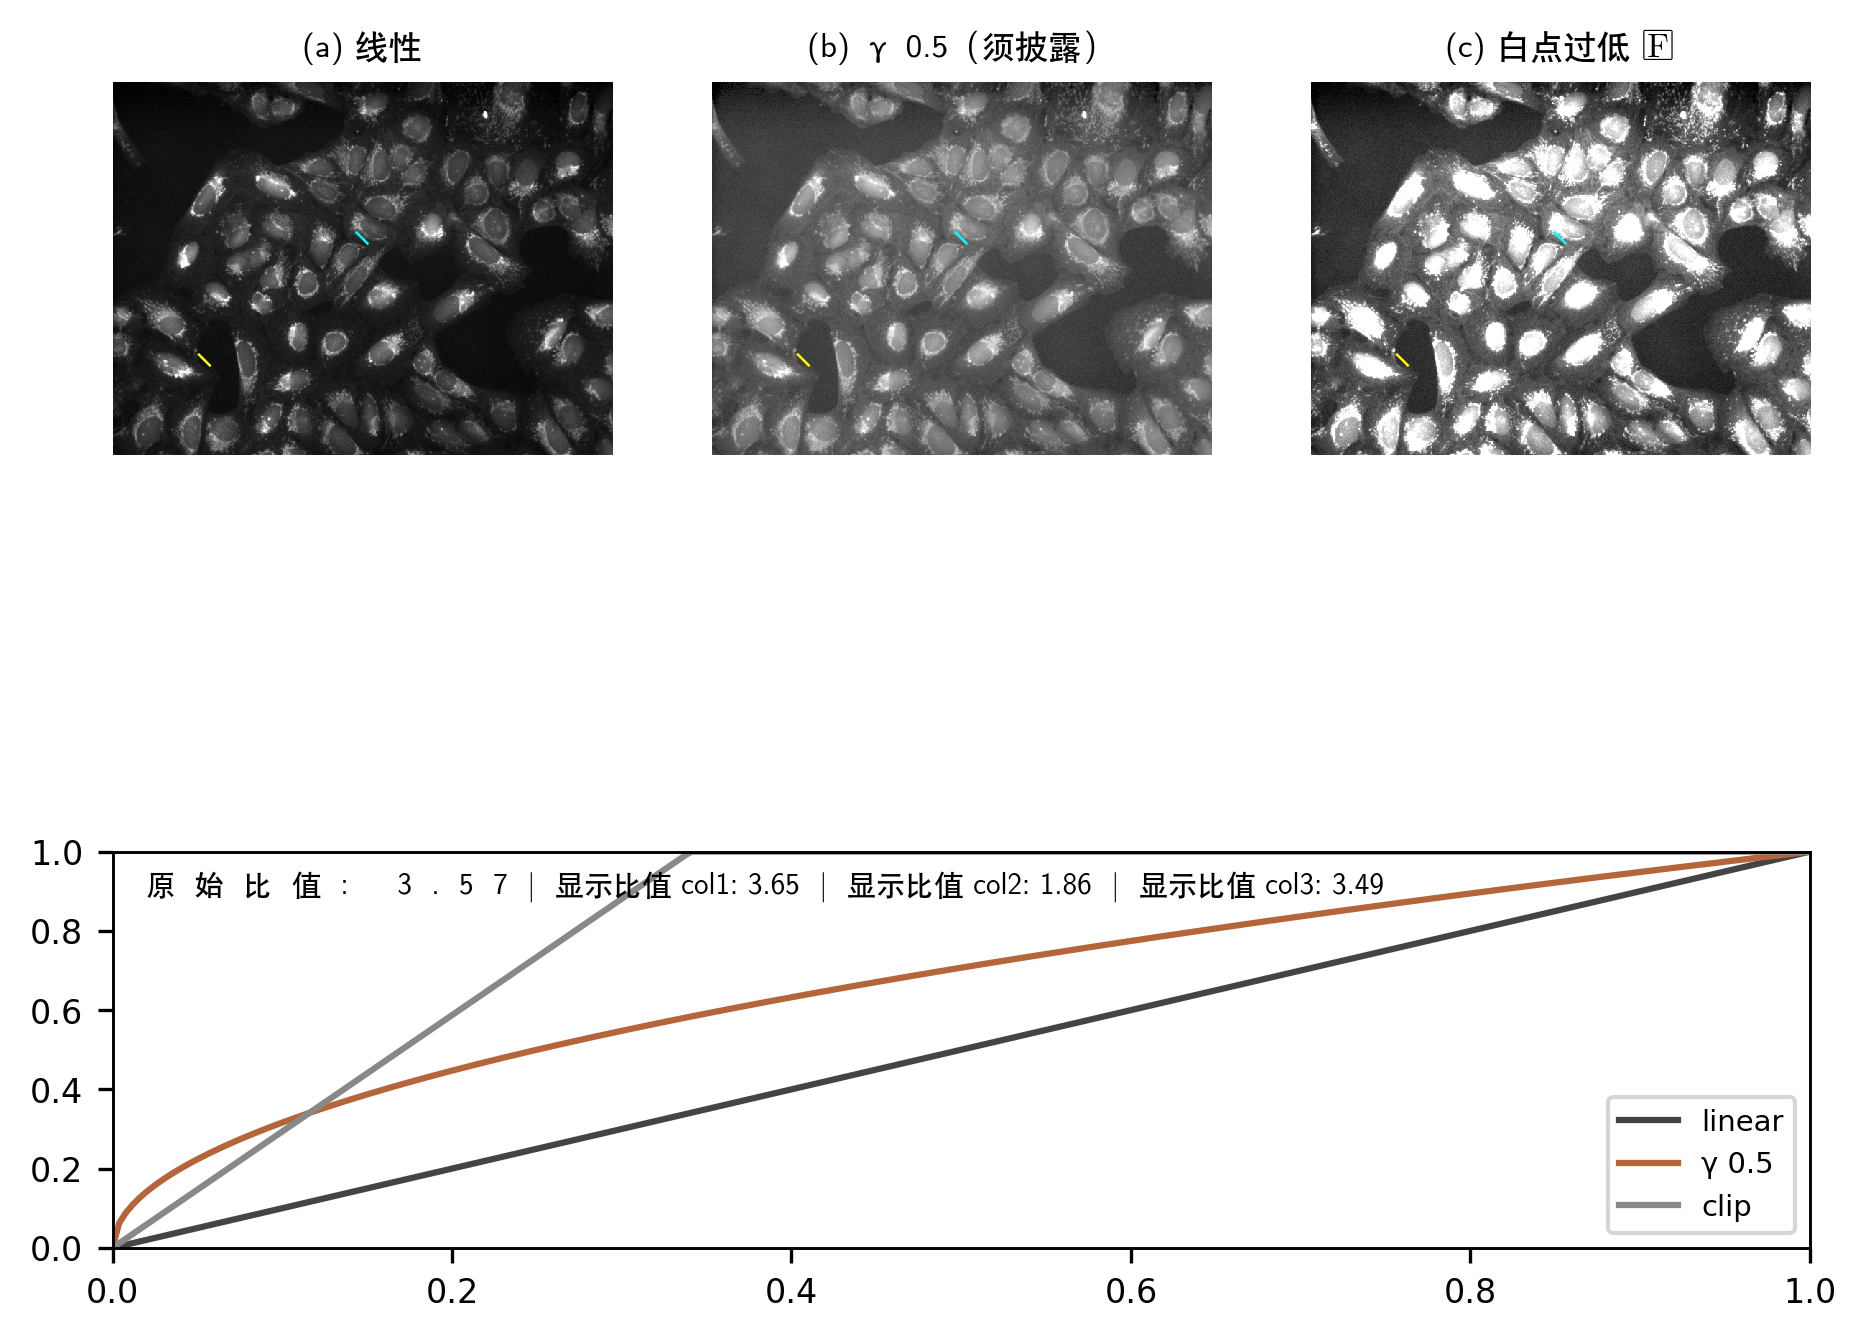
\includegraphics[width=0.88\linewidth]{figures/ch08/ch08-02-linear-vs-gamma-zh.png}
\caption{线性与非线性显示的区别。(a) 线性映射（$218\text{--}1140$）。(b) 同一图像施加 $\gamma = 0.5$，暗部信号变亮，亮暗区域的相对强度随之改变；这种调整必须在图注中披露。(c) 反例：白点过低导致大部分线粒体信号被截断为纯白，信息丢失。下方曲线为三种映射，并列出两个固定区域（青色与黄色短线）的原始强度比与显示灰度比。图像：BBBC022v1，CC0。}\label{fig:ch08-02}
\end{figure}

观察图~\ref{fig:ch08-02} 的三列画面与下方传递曲线：
\begin{enumerate}
\item \textbf{面板 (a)（线性映射 $218\text{--}1140$）：}核周线粒体簇与胞质远端细丝层次分明；亮、暗两处 ROI 的 8 位显示灰度比值为 $3.65$（\texttt{col1: 3.65}），与原始比值 $3.57$ 仅差 8 位整数舍入带来的微小偏差，真实保持了亮暗相对比例。
\item \textbf{面板 (b)（$\gamma = 0.5$，黑白点仍为 $218\text{--}1140$）：}下方棕色曲线向上拱起，胞质外周弱信号明显变亮，但两处 ROI 的显示灰度比值从 $3.57$ 降至 $1.86$（\texttt{col2: 1.86}），相对差距缩水近半。若不在图注中披露 $\gamma = 0.5$，读者就会误判信号的空间分布比例。
\item \textbf{面板 (c)（反例，白点设为第 $90\%$ 分位数 $532$）：}下方灰色折线在横轴约三分之一处即触顶封平，全图有 \textbf{$9.94\%$ 的像素被截断为纯白（$255$）}。尽管此时两个 ROI 的均值比读作 $3.49$（\texttt{col3: 3.49}，因为更陡的直线斜率在把亮区顶死在 $255$ 的同时，也把暗区同步拉高了），但画面上几乎所有核周线粒体都变成了刺眼的实心白斑，内部结构彻底丢失。
\end{enumerate}

\textbf{第三，严禁阈值化抹黑背景、局部涂抹或使用克隆修复工具。}无论是单独提亮某几颗细胞，还是用仿制图章（clone stamp）、修复画笔抹掉荧光杂质或背景斑点，都属于篡改原始测量数据（Rossner 与 Yamada，2004；Cromey，2010）。

\textbf{第四，同一组比较中的所有面板，必须使用完全相同的显示设置。}如果对每个面板分别点“自动对比度”，真实的处理效应会被抵消，而原本没有差异的对照视野却能被调出假差异。图~\ref{fig:ch08-03} 用同一对照孔（A13 孔，DMSO 对照）的两个相邻视野 \texttt{s1} 与 \texttt{s2}（线粒体通道）演示了这一后果：右侧柱状图计算了两幅 16 位原图的全幅平均强度，\texttt{s1} 为 $373.2\ \text{a.u.}$，\texttt{s2} 为 $366.3\ \text{a.u.}$，相差不到 $2\%$（注：每视野仅一个均值，此处仅用于核对原始量级，不是统计检验）。

\begin{figure}[htbp]\centering
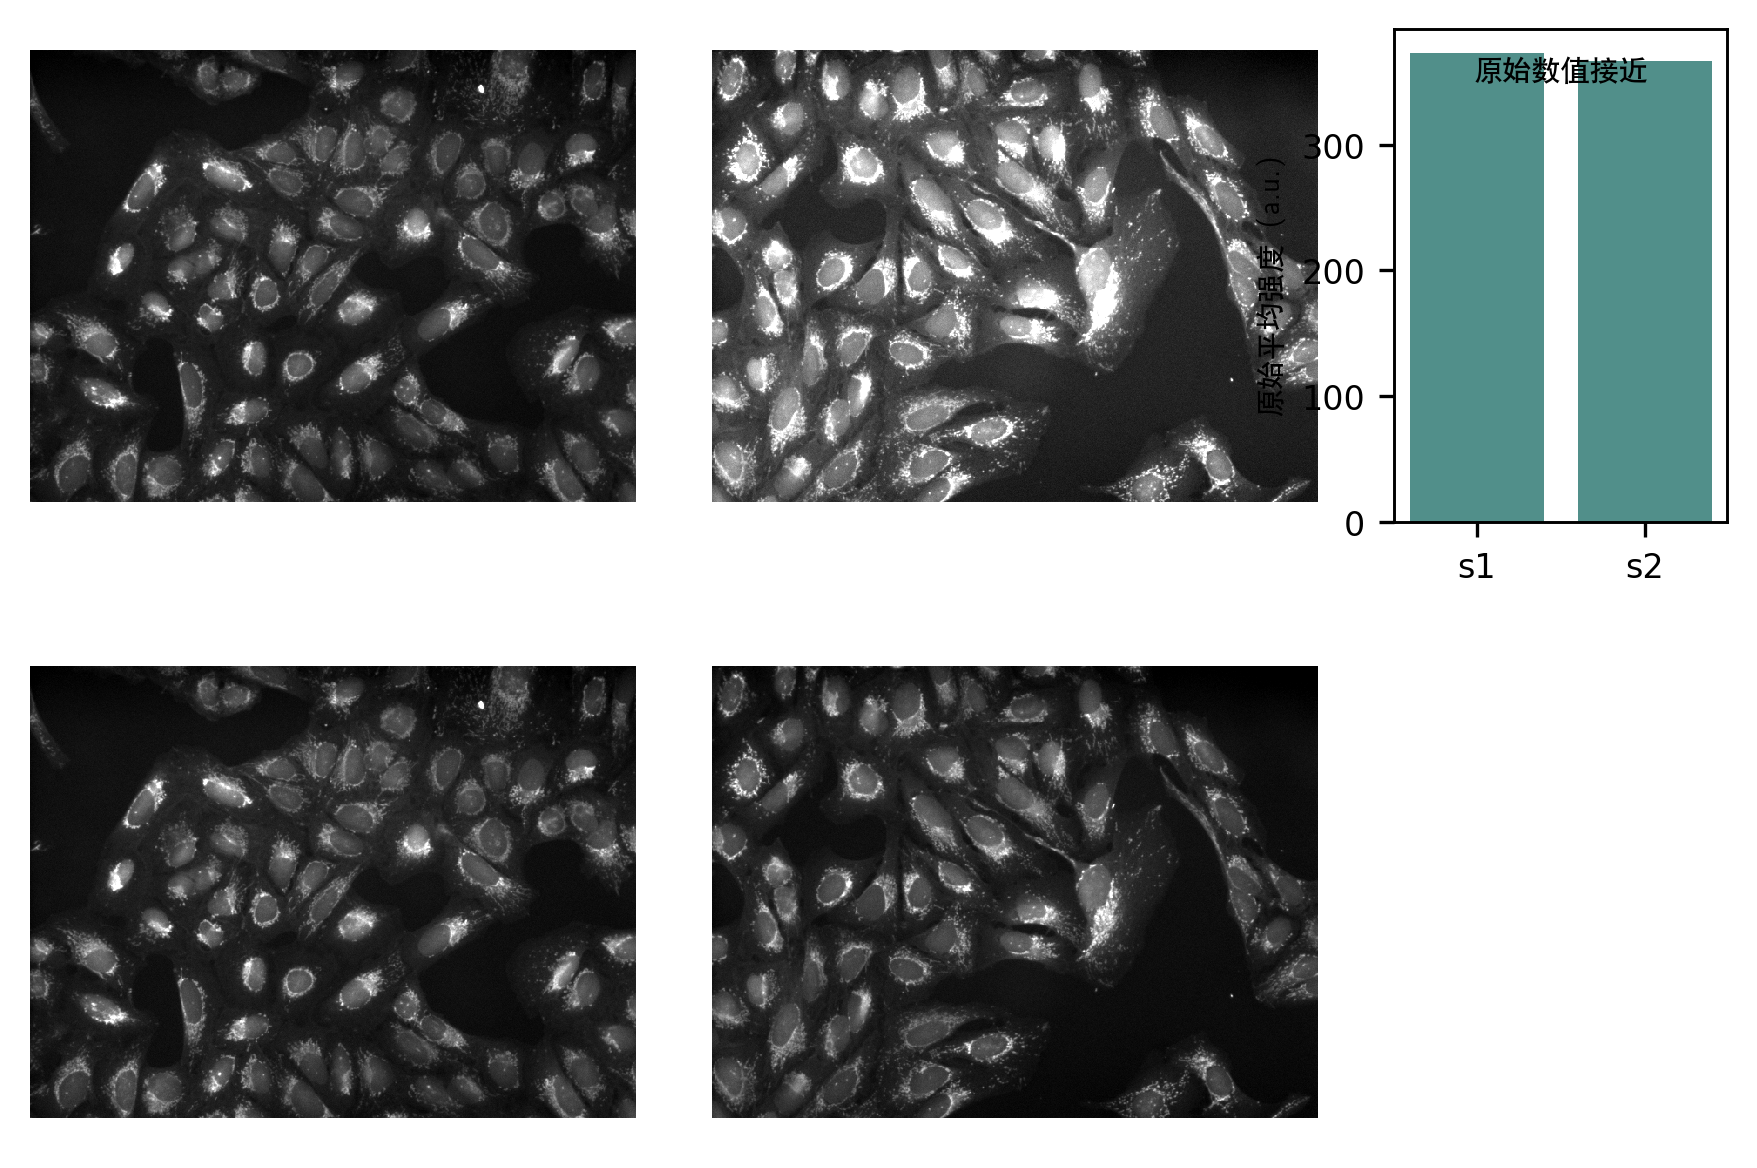
\includegraphics[width=0.88\linewidth]{figures/ch08/ch08-03-consistent-display-zh.png}
\caption{比较面板必须使用相同的显示设置。两幅图来自同一对照孔（BBBC022，孔 A13，视野 1 与 2），没有处理差异。上排分别设置显示范围，右图看似信号更强；下排使用同一显示范围（$218\text{--}1140$），差异消失。右侧为两视野原始平均强度。上排右图的显示范围为教学反例而刻意设定。图像：BBBC022v1，CC0。}\label{fig:ch08-03}
\end{figure}

看图~\ref{fig:ch08-03} 上排的反例：左图 \texttt{s1} 按 $218\text{--}1140$ 映射，右图 \texttt{s2} 刻意将白点压低为 $196\text{--}700$。仅仅因为白点降低了不到四成，上排右图的线粒体就大面积泛白发亮，看似比左图信号强得多；而在下排改用统一的显示范围（$218\text{--}1140$）后，两视野的亮度与染色模式立刻恢复一致。

\section{通道与伪彩色}

荧光显微镜相机对每个波段采集的都是单通道灰度图，论文里看到的彩色是作者指定的伪彩色查找表（LUT）。选择伪彩色时需遵循三条规则：

\textbf{第一，避免红/绿合成，改用品红/绿（或青/品红/黄），并优先提供分通道灰度面板。}男性读者中约有 $8\%$ 存在红绿色觉异常（Wong，2011；Crameri 等，2020）。在传统的红/绿合成图中，纯红与纯绿在红绿色盲读者眼中都会投射为相近的黄褐色，不仅两通道彼此难以区分，连代表共定位的黄色也会融进背景。把红色替换为\textbf{品红色（magenta，将同一通道同时写入红通道 R 与蓝通道 B）}、保留另一通道为\textbf{绿色（写入绿通道 G）}后，第一通道含有强烈的短波蓝光分量，两通道重叠处则叠加为高对比度的白色（$R+G+B$），在两类红绿色盲眼中都能清晰分辨。同时，人眼对单通道灰度的空间细节分辨力高于彩色图（Jambor 等，2021；Schmied 与 Jambor，2020），“分通道灰度 + 品红/绿合成”是最稳妥的组合。

图~\ref{fig:ch08-04} 截取第 1 视野的 $300 \times 300$ 像素区域（坐标 $(198, 110)\text{--}(498, 410)$，显示范围固定为细胞核 $132\text{--}1236$、线粒体 $218\text{--}1140$），在线性 RGB 空间采用 Machado 等（2009）模型（严重度 $1.0$）模拟色觉异常效果。

\begin{figure}[htbp]\centering
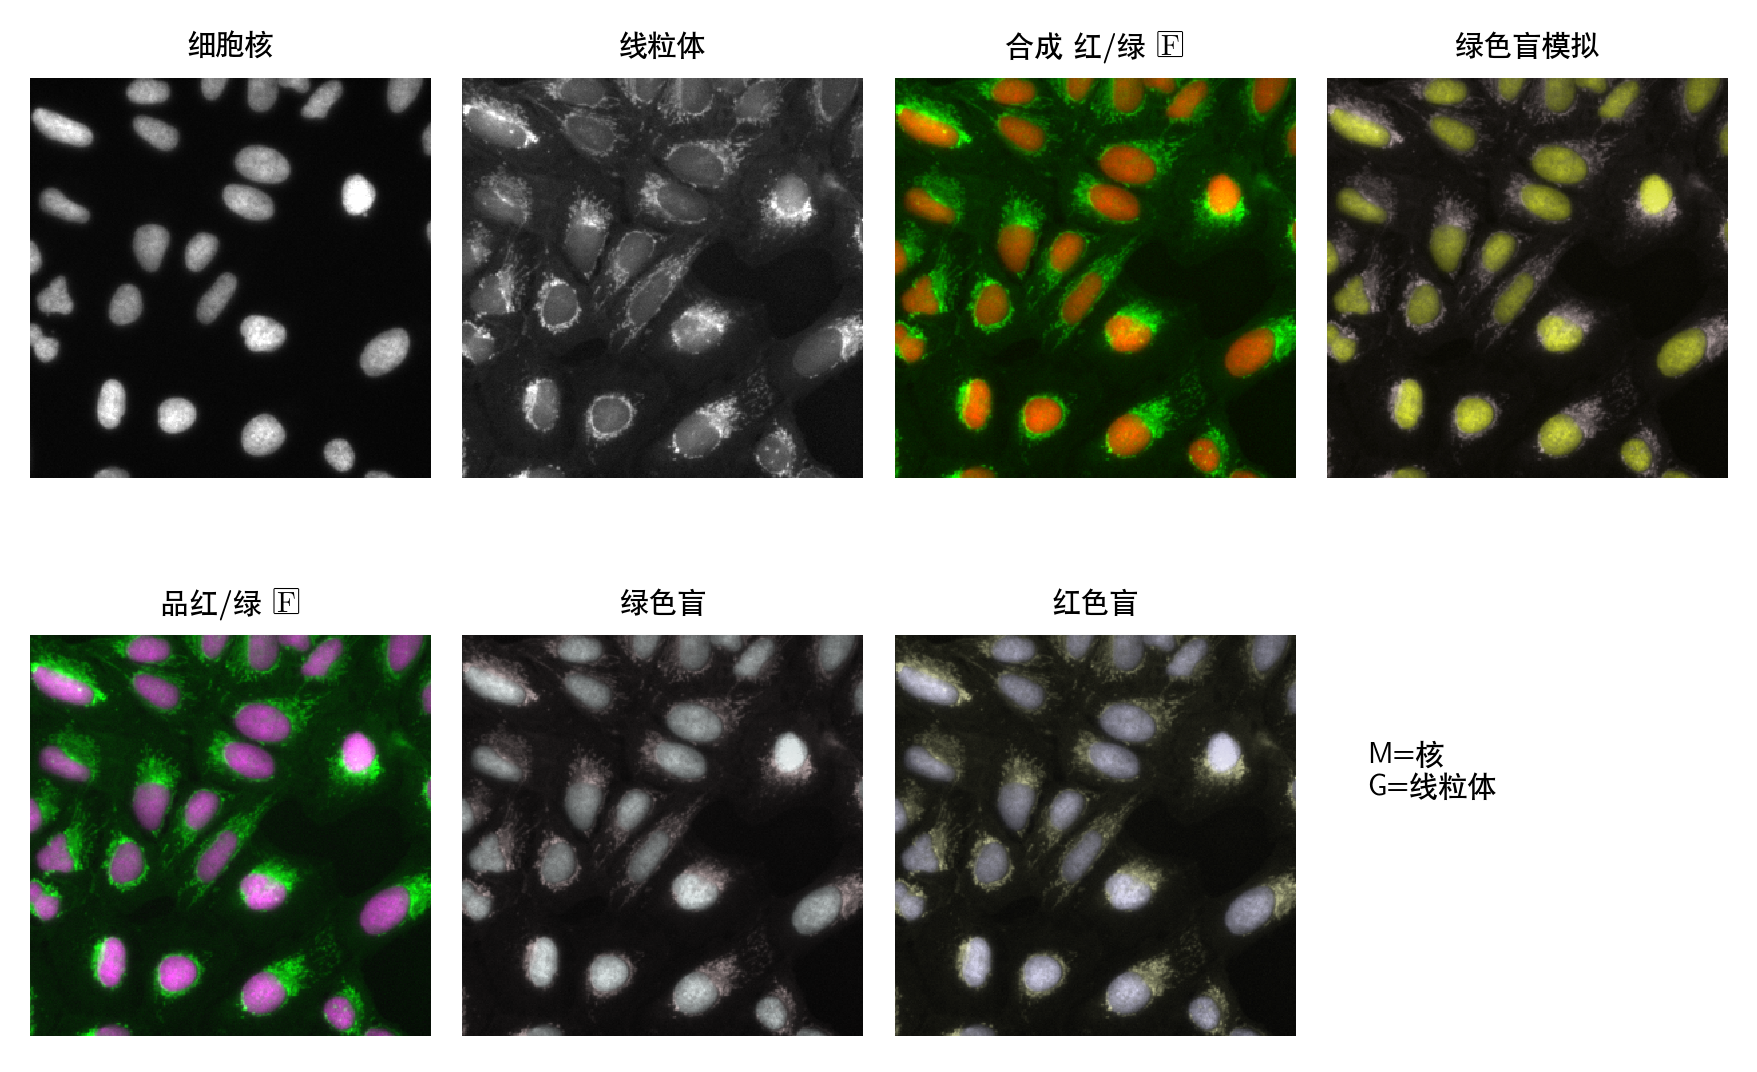
\includegraphics[width=0.88\linewidth]{figures/ch08/ch08-04-pseudocolor-colorblind-zh.png}
\caption{多通道荧光图的伪彩色选择。上排：红/绿合成在绿色盲模拟下两通道难以区分。下排：品红/绿合成在绿色盲与红色盲模拟下仍可区分。单通道灰度图不依赖颜色辨别。色觉模拟采用 Machado 等（2009）模型。图像：BBBC022v1，CC0。}\label{fig:ch08-04}
\end{figure}

对比图~\ref{fig:ch08-04} 上下两排：上排左三的红/绿合成在绿色盲模拟（上排右一）下，细胞核与核周线粒体全部变成相近的暗黄绿色，边界难以剥离；而下排左一的品红/绿合成在绿色盲（下排左二）与红色盲（下排左三）模拟下，浅灰紫色的细胞核与暖橄榄色的线粒体依然界限分明。导出成图后，还可用 \scidraw{} 的图片检查工具（\sdtool{figure-checker}）对整图做色觉风险复查。

\textbf{第二，合成前各通道单独设定线性显示范围并逐一记录。}Nature Portfolio 图像诚信政策规定，合成图中若对单通道做过独立调整须在图注说明。在脚本中先对各 16 位通道按固定 $(v_{\min}, v_{\max})$ 映射为 8 位灰度再合成 RGB，合成后不再做整图调色，即可准确记录并披露参数。

\textbf{第三，扫描电镜（SEM）原本无颜色，人工上色属于伪彩，必须明确声明。}电子显微镜记录的是电子通量强度，原始图像只有灰度。例如达特茅斯学院电镜中心发布在公有领域的混合花粉 SEM 图，原版（\url{https://commons.wikimedia.org/wiki/File:Misc_pollen.jpg}，$1228 \times 935$ 像素）为灰度图，而彩色版（\url{https://commons.wikimedia.org/wiki/File:Misc_pollen_colorized.jpg}）是后期按颗粒轮廓人工涂上的伪彩。作为实验证据呈现时，SEM 图应保持原始灰度；若因说明需要施加伪彩，必须在图注中明确声明。

\section{裁剪、放大与比例尺}

\subsection{保持含义的裁剪与局部放大}

裁剪选区不能变成“挑视野里最亮、最好看的一颗细胞”（Cromey，2010；Jambor 等，2021）。规范的裁剪与局部放大需满足四项要求：
\begin{enumerate}
\item \textbf{选有代表性的区域并写明依据：}例如在展示对照视野时，选取细胞核与线粒体强度均处于视野中位数附近的典型区域，并将选择依据写入处理记录。
\item \textbf{记录精确裁剪框坐标：}将裁剪框在原图中的像素坐标 $(x_0, y_0, x_1, y_1)$ 保存到处理记录中。
\item \textbf{局部放大在母图上标出位置，并优先采用整数倍最近邻插值：}在母图对应位置画出方框（共用同一组像素坐标），写明放大倍数（如 $3\times$）。放大像素块时推荐使用\textbf{最近邻插值（nearest-neighbour）}，把每个原始像素原样扩展为 $3 \times 3$ 同色方块，如实展现相机的空间采样极限，而不使用双三次（bicubic）插值伪造平滑边缘，更不允许“补细节”。
\item \textbf{禁止无缝拼接：}不同视野、时间点或凝胶泳道的图像不得拼成“同一视野”；确需并列须加清晰分隔线并在图注中说明（Rossner 与 Yamada，2004；Bik 等，2016）。
\end{enumerate}

\subsection{从校准信息计算比例尺}

比例尺像素长度等于目标物理长度除以像素物理尺寸：$L_{\text{px}} = L_{\text{phys}} / s_{\text{px}}$；若放大面板做了 $k$ 倍放大，则比例尺像素长度需乘以 $k$ 重新计算：$L'_{\text{px}} = (L'_{\text{phys}} / s_{\text{px}}) \times k$。像素物理尺寸 $s_{\text{px}}$ 只能来自采集元数据、同期拍摄的标准测微尺，或原图底部的\textbf{仪器数据条}。

图~\ref{fig:ch08-05} 以达特茅斯学院电镜中心 Louisa Howard 拍摄的美洲烟草（\textit{Nicotiana alata}）叶片上表皮 SEM 原图（\path{Leaf_epidermis.jpg}，公有领域，$2048 \times 2073$ 像素，8 位灰度）演示比例尺换算、裁剪与局部放大。

\begin{figure}[htbp]\centering
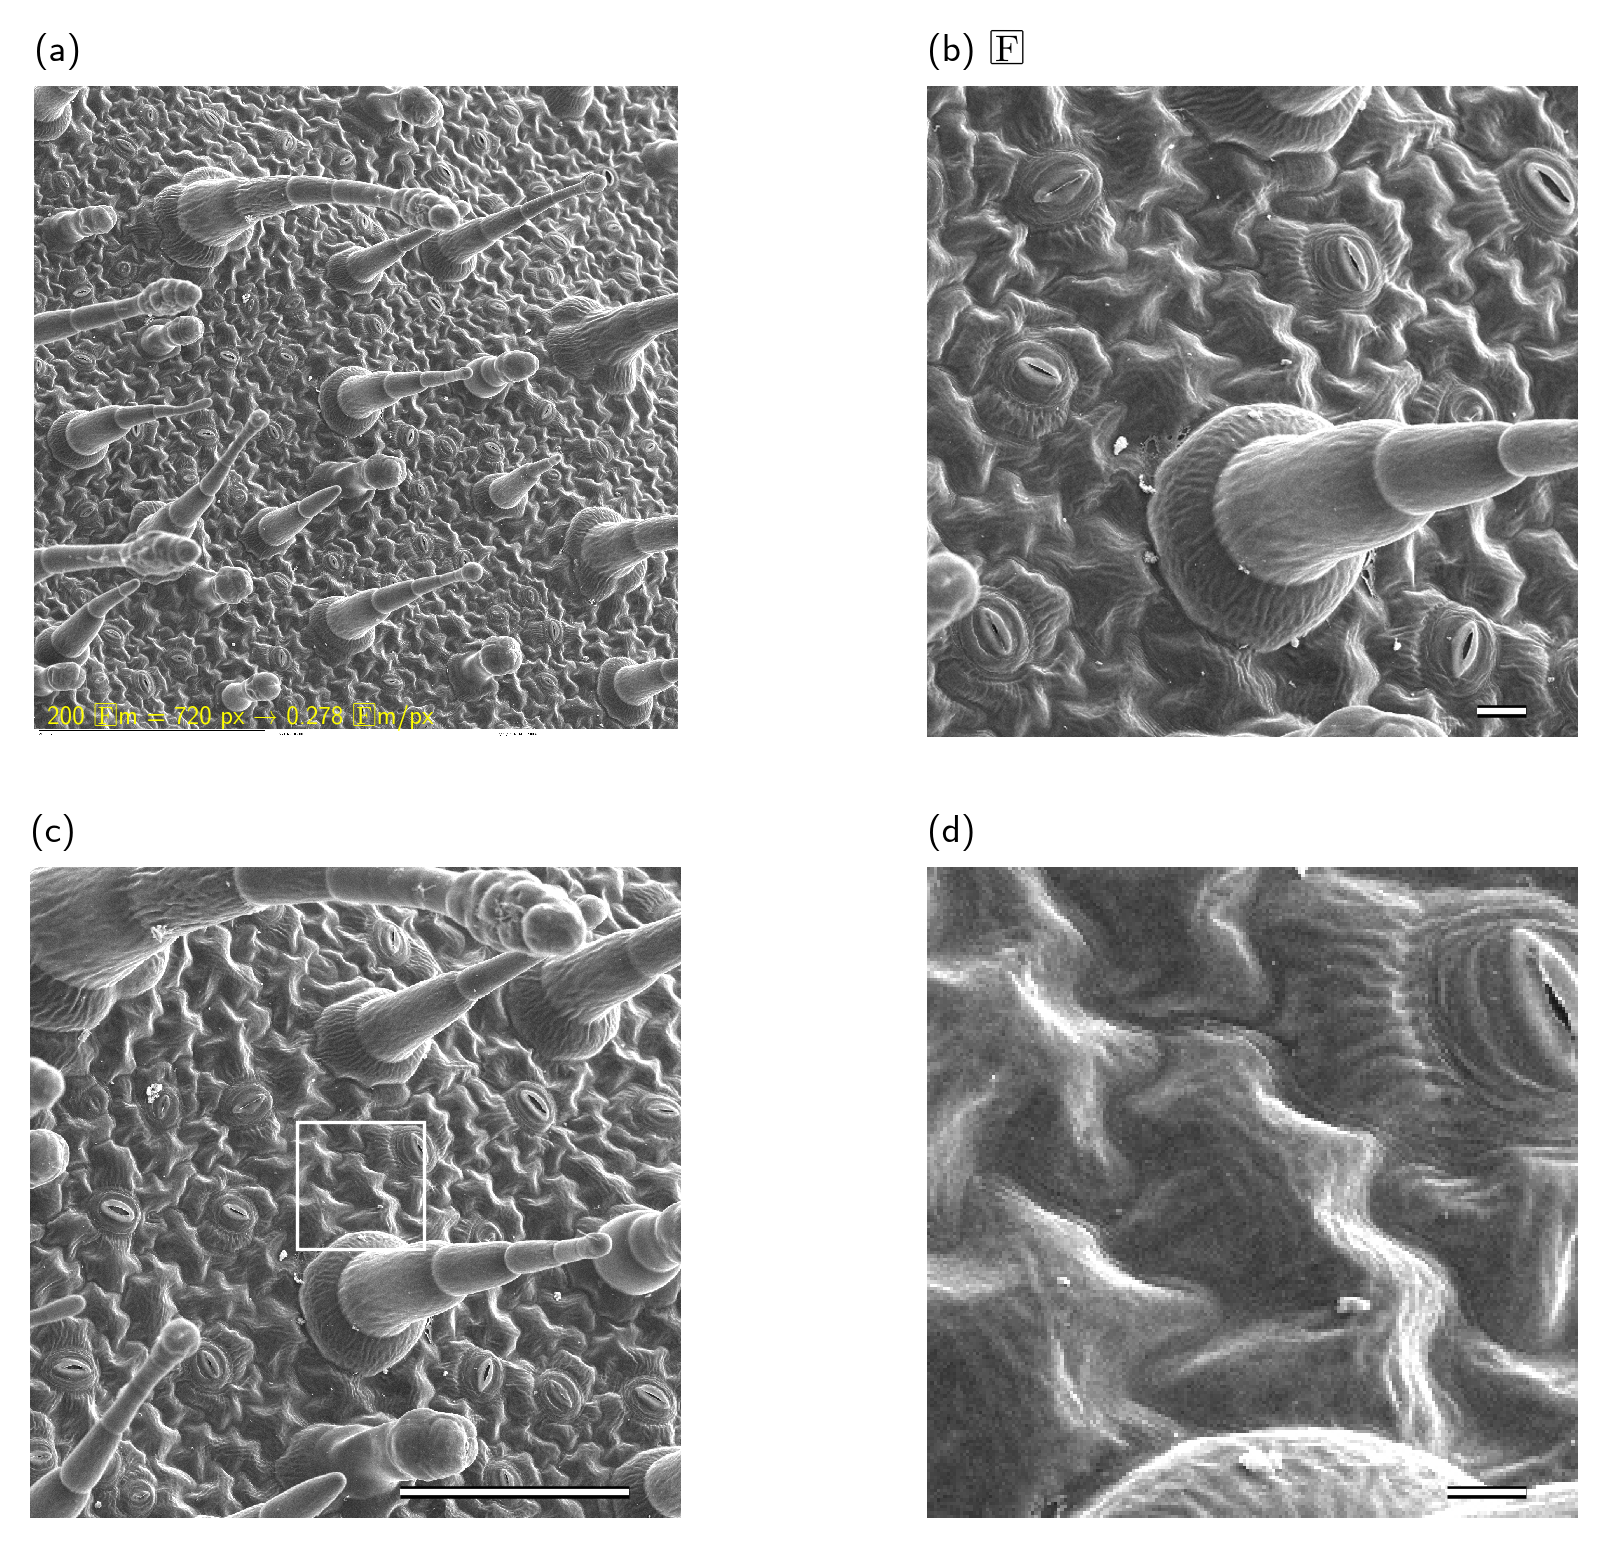
\includegraphics[width=0.88\linewidth]{figures/ch08/ch08-05-crop-inset-scalebar-zh.png}
\caption{裁剪、局部放大与比例尺。(a) 原始 SEM 图像（\textit{Nicotiana alata} 叶上表皮，Zeiss 962，$200\times$），底部为仪器数据条；其中 $200\ \mu\text{m}$ 标尺线长 $720$ 像素，据此像素尺寸为 $0.278\ \mu\text{m}$。(b) 反例：裁掉数据条、只保留个别结构、以双三次插值放大并画上无依据的比例尺。(c) 正确做法：记录裁剪框，按像素尺寸绘制 $100\ \mu\text{m}$ 比例尺；白框区域在 (d) 中以 3 倍最近邻放大，比例尺 $20\ \mu\text{m}$。图像：Louisa Howard, Dartmouth Electron Microscope Facility，公有领域。}\label{fig:ch08-05}
\end{figure}

对照图~\ref{fig:ch08-05} 的四个面板：
\begin{itemize}
\item \textbf{面板 (a)（从原图仪器数据条实测像素尺寸）：}原图底部 $25$ 行像素（行号 $2048\text{--}2072$）为蔡司 DSM 962 电镜自动生成的白色数据条，印有标尺线及“\texttt{200 um}”“\texttt{200X}”“\texttt{7/31/3 REMF}”“\texttt{Nict.\ leaf \#2.001}”。脚本自动扫描数据条区域的水平暗像素连续游程（灰度 $<80$），测得第 $2052\text{--}2053$ 行、$x = 15\text{--}734$ 的黑色标尺线精确跨越 \textbf{$720$ 像素}，由此算得 $s_{\text{px}} = 200\ \mu\text{m} / 720\ \text{px} \approx 0.2778\ \mu\text{m/px}$（依赖仪器放大率标定，图注写明“据仪器数据条换算”）。此外，Wikimedia Commons 上另有第三方裁掉数据条并另加“$200\ \mu\text{m}$”白线的派生图（\path{Leaf_epidermis_w_scale.jpg}，$2048 \times 2052$ 像素）。使用第三方派生图时必须回到原图核对——我们实测该派生图白线（$x=240\text{--}959$）长 $720$ 像素，与原图数据条一致，这就是“回原图核对”的示范。
\item \textbf{面板 (b)（反例）：}裁掉底部数据条，只截取中央一根毛状体（$600 \times 600$ 像素）做 $4\times$ 双三次插值放大，并在右下角随手画了一根标称“$50\ \mu\text{m}$”、实为正确换算长度 2 倍的无依据比例尺。
\item \textbf{面板 (c) 与 (d)（正确做法）：}面板 (c) 记录 $1024 \times 1024$ 像素裁剪框 $(480, 320)\text{--}(1504, 1344)$，绘制 $100\ \mu\text{m} = 360\ \text{px}$ 比例尺，并用白框标出 $200 \times 200$ 像素的气孔区域 $(900, 720)\text{--}(1100, 920)$；面板 (d) 将白框区域做 $3\times$ 最近邻放大，比例尺按放大倍数重算为 $20\ \mu\text{m} = 72 \times 3 = 216\ \text{px}$。
\end{itemize}

\subsection{没有校准信息就不画比例尺}

如果图像没有记录像素尺寸，也没有仪器数据条，唯一合规的做法是\textbf{不画比例尺，并在图注中写明“像素尺寸未知”}——绝不能按“细胞看起来大约 $20\ \mu\text{m}$”去估画。

图~\ref{fig:ch08-06} 展示了来自 ImageJ 示例集的三通道荧光图（\path{FluorescentCells.jpg}，牛肺动脉内皮细胞，蓝 DAPI、绿微管、红 F-actin，公有领域，$512 \times 512$ 像素；同时也是第 3 节红/绿共存合成的反例）：该文件以 8 位有损 JPEG 合成图发布，JFIF 密度为无单位的 $1:1$，来源页未给物镜与像素尺寸（面板 a）。面板 (b) 凭印象加比例尺属于编造尺度；面板 (c) 不画比例尺并标明“未校准”才是正确做法；面板 (d) 将局部 $(200, 200)\text{--}(280, 280)$ 做 $4\times$ 最近邻放大，清晰可见 $8 \times 8$ JPEG 块状伪影与通道串色，说明该文件只能作为定性显示图，不能当作原始测量数据。

\begin{figure}[htbp]\centering
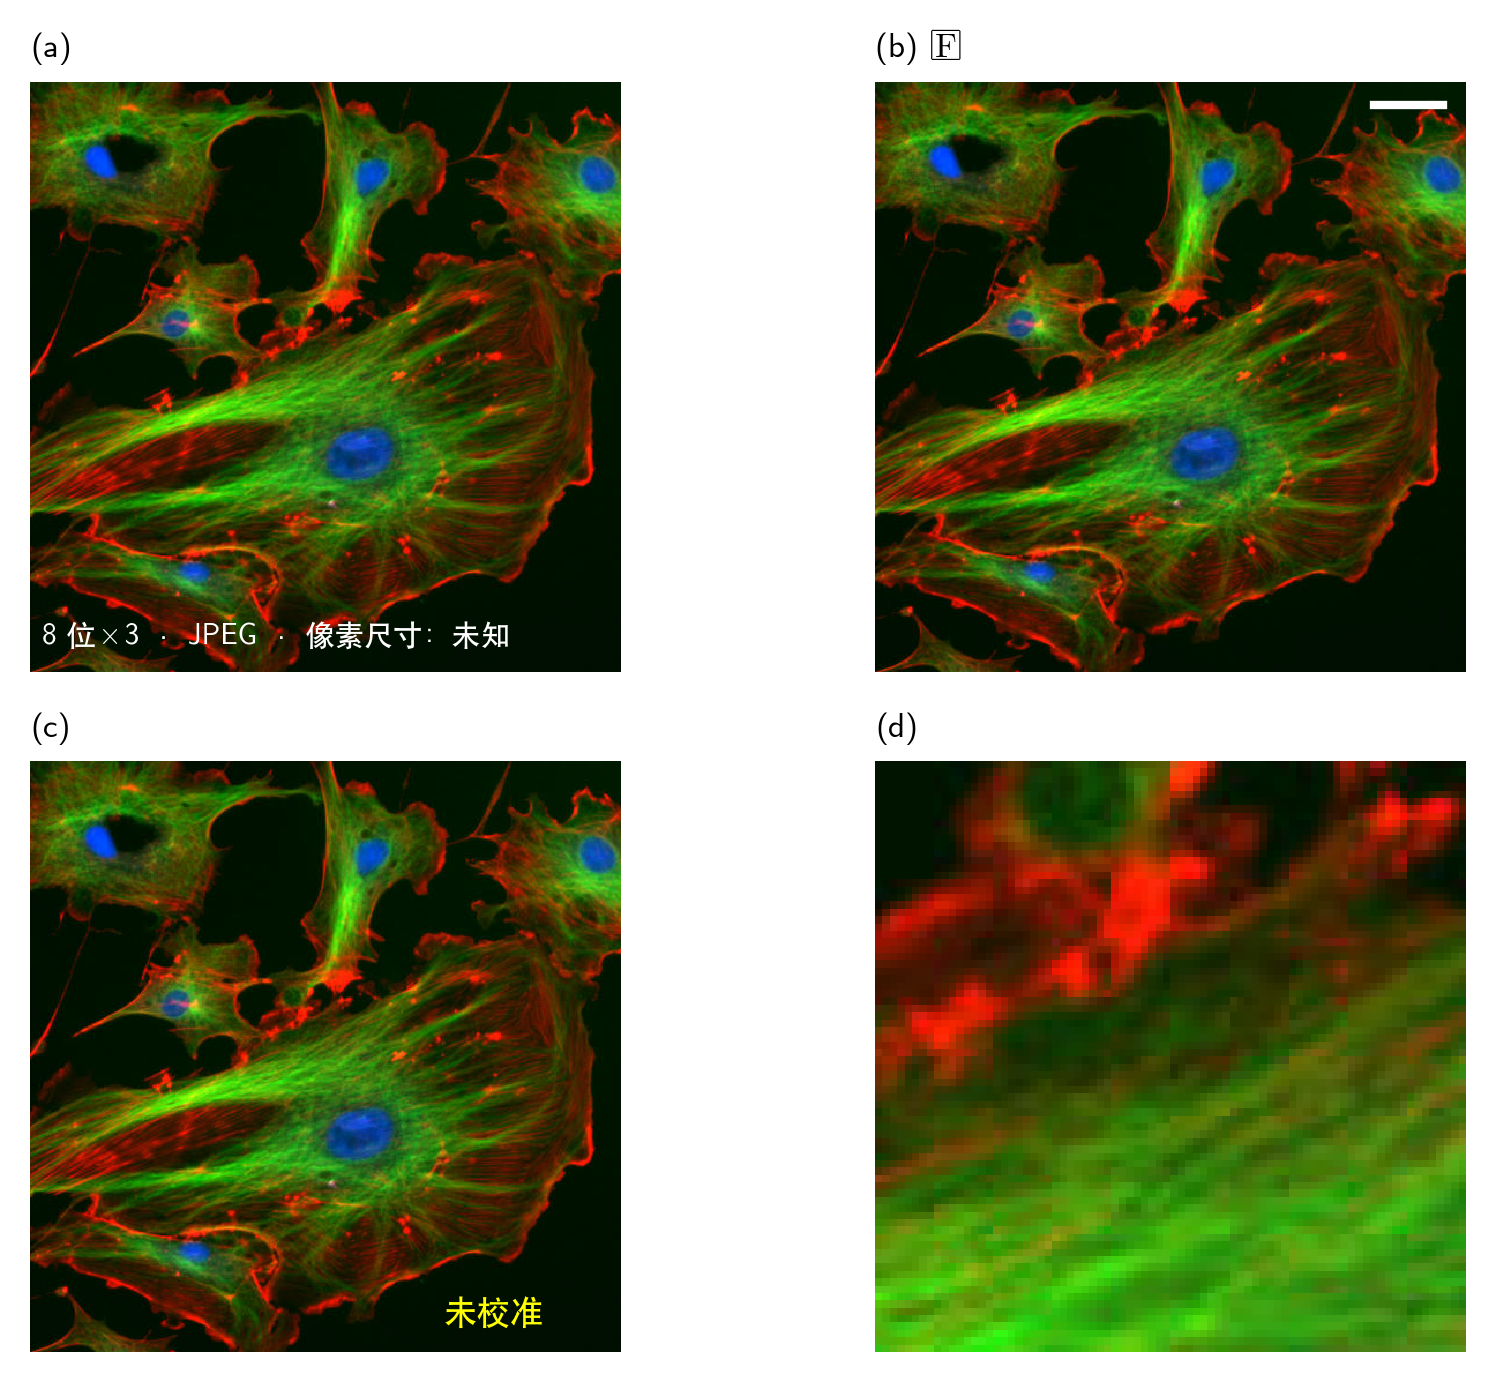
\includegraphics[width=0.88\linewidth]{figures/ch08/ch08-06-no-calibration-zh.png}
\caption{没有校准信息时不画比例尺。(a) 来自 ImageJ 示例集的三通道荧光图（牛肺动脉内皮细胞；蓝 DAPI、绿微管、红 F-actin），以 8 位 JPEG 合成图发布，未记录像素尺寸。(b) 反例：凭印象添加的比例尺。(c) 正确做法：不画比例尺，并在图注中写明“像素尺寸未知”。(d) 局部放大可见 JPEG 压缩块，说明此文件只能作为显示图，而不是原始测量数据。图像：公有领域（Wikimedia Commons，FluorescentCells.jpg）。}\label{fig:ch08-06}
\end{figure}

\section{期刊规则与 AI 的边界}

\textit{Journal of Cell Biology}（Rossner 与 Yamada，2004）提出的经典规则与 Cromey（2010）的伦理准则共同确立了科学数字图像的底线：整图调整亮度、对比度或色彩平衡是可接受的（非线性调整须在图注披露），但\textbf{图像中的任何特定特征均不得被增强、遮蔽、移动、移除或引入}。Bik 等（2016）对 20,621 篇生物医学论文的筛查发现约 $3.8\%$ 存在不当图像重复或操作，促使主流期刊在出版前全面引入图像取证检查。

在生成式 AI 时代，Nature Portfolio《图像诚信与标准》与 Springer Nature《人工智能（AI）政策》（均于 2026 年 10 月 29 日访问；该政策更新频繁，正文引用与投稿前均须核对最新文本）进一步规定：调整须整图且对照同等施加，不得让数据消失，伪彩与 $\gamma$ 等非线性调整以及合成图中的单通道调整均须在图注说明，禁止克隆与修复工具，并把\textbf{“伪造数据、引用或结果”与“生成照片级图像（deepfakes）”明确列为不允许}。

为什么不能把模糊的实验图像交给生成式模型“去噪、变清晰”？我们在图~\ref{fig:ch08-05} 所用的烟草叶表皮 SEM 原图上做了一个有真实地面真值（GT）的对照实验（图~\ref{fig:ch08-07}）：
\begin{enumerate}
\item 从原图截取 $512 \times 512$ 像素区域 $(640, 680)\text{--}(1152, 1192)$ 作为\textbf{地面真值 GT}（面板 a），内含三处气孔、表皮细胞边界、右侧大毛状体基部与左下斜向小毛状体。
\item 按 $4 \times 4$ 区域平均降采样为 $128 \times 128$ 像素低分辨图 \textbf{LR}（面板 b，最近邻显示）。
\item \textbf{对照 1（面板 c）：}将 LR 用双三次插值放大回 $512 \times 512$ 像素（确定性插值，模糊但不添加新结构）。
\item \textbf{对照 2（面板 d）：}将同一张 $128 \times 128$ 的 LR 图传入图像生成模型的编辑模式，按普通用户常见的英文提示词独立运行 3 次（为避免挑选最离谱的一次，正文固定使用第 1 次结果，其余两次存档）：
\end{enumerate}

\begin{Prompt}
Upscale this grayscale scanning electron microscope image to 512 x 512 pixels.
Make it sharper and more detailed, remove blur and noise, and enhance the fine
surface structures so it looks like a high-resolution micrograph.
Keep it grayscale. Do not add any text, letters, numbers, labels, or scale bars.
Square 1:1 aspect ratio.
\end{Prompt}

\begin{figure}[htbp]\centering
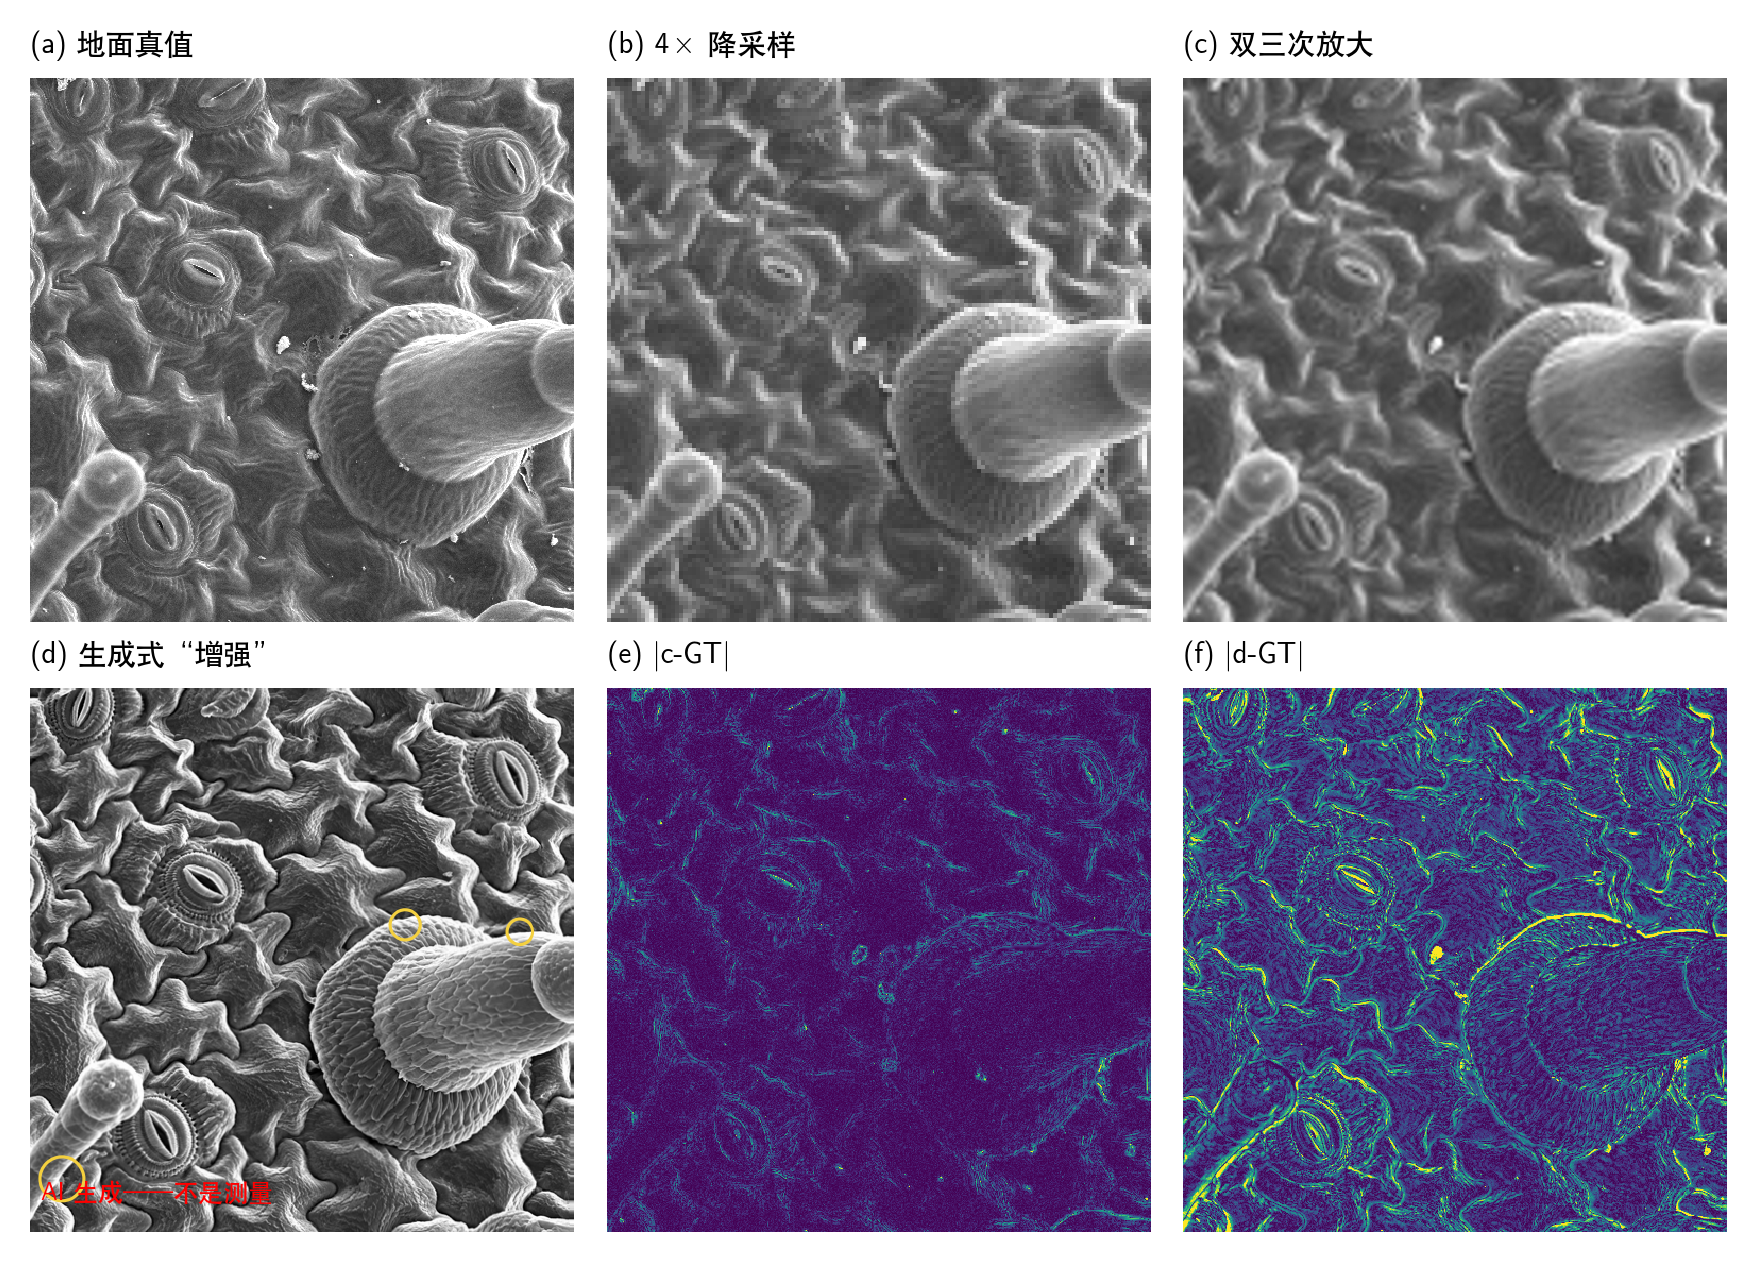
\includegraphics[width=0.88\linewidth]{figures/ch08/ch08-07-generative-risk-zh.png}
\caption{生成式“增强”会编造结构。(a) SEM 原图局部（地面真值）。(b) 将其 4 倍降采样后的低分辨率版本。(c) 双三次插值放大：图像模糊，但没有新增结构。(d) 用图像生成模型按“变清晰、增强细节”的要求放大：看起来更清晰，却含有原图中不存在的边界与纹理（圆圈处）。(e)、(f) 分别为 (c)、(d) 与原图的绝对差。生成图仅用于说明风险，不能作为实验图像使用。原图：Louisa Howard, Dartmouth Electron Microscope Facility，公有领域；面板 (d) 由图像模型生成，提示词与生成记录见本书仓库。}\label{fig:ch08-07}
\end{figure}

对比图~\ref{fig:ch08-07} 的六个面板与三次生成结果，可以看到生成式“增强”的四重失真（本实验不评测某一特定产品，任何生成式放大模型都有同类风险）：
\begin{itemize}
\item \textbf{像素尺寸与通道属性失控：}提示词明确要求输出 $512 \times 512$ 单通道灰度图，但三次调用实际返回的全部是 $1254 \times 1254$ 像素（约为输入边长 $9.8$ 倍）的三通道 8 位 RGB 图，且 RGB 三通道间存在最大 $10\text{--}12$ 灰阶的差值，并非严格单通道灰度。
\item \textbf{凭空捏造原图中不存在的边界与纹理：}面板 (d) 看似比双三次插值 (c) 清晰得多，但与地面真值 (a) 逐区对照可见：左上气孔开口外围被编造出规则的多层环形边缘与齿状纹理，右侧大毛状体及表皮铺满了原图并不存在的紧密鳞片状细纹；在面板 (d) 用三个黄色圆圈标出的位置——大毛状体基部上缘的两处褶皱脊线（中心约 $(353, 222)$ 与 $(460, 229)$）和左下小毛状体顶端（中心约 $(30, 461)$）——模型均画出了原图中不存在的亮边与结构边界。
\item \textbf{多次生成之间细节互相矛盾：}同一张 $128 \times 128$ 输入图独立生成三次，第 1 次表面是紧密条片纹，第 2 次变成更圆钝密集的卵石状颗粒且左下毛状体顶端裂成多边形分块，第 3 次又在大毛状体基部画出放射状细长褶片。这证明新出现的高频细节并非来自样品测量，而是模型随机填充的纹理。
\item \textbf{逐像素绝对误差接近双三次插值的 3 倍：}将第 1 次生成输出转为灰度、仅因比较需要用 Lanczos 缩回 $512 \times 512$，再做一次刚性配准（旋转 $-0.5^\circ$，平移 $dx=-1, dy=+1$ 像素）以消除轻微几何错位，计算与地面真值 GT 的绝对差（面板 e、f，统一采用 $0\text{--}128$ 的 \texttt{viridis} 色标）。双三次插值 $|c - \text{GT}|$（面板 e）的平均绝对误差（MAE）仅为 $10.32$ 灰阶；而生成式放大 $|d - \text{GT}|$（面板 f）配准后的 MAE 高达 $28.91$ 灰阶（配准前为 $29.06$），画面布满亮黄与亮绿色误差带。
\end{itemize}

结论只有一条：\textbf{AI 可以帮你写处理脚本、写方法、查色觉，但不能产生任何一个将被当作测量的像素。}

\section{完整案例：U2OS 细胞对照视野的呈现}

现在我们把小苏的补充材料方法图完整走一遍。本图用于在论文补充材料中展示 DMSO 对照（\texttt{mock}）条件下 U2OS 细胞的细胞核与线粒体染色模式，让同行判断后续定量分析所用原始图像的质量。本图\textbf{不报告任何处理效应}；由于使用公开基准数据集 BBBC022v1（Gustafsdottir 等，2013），采集参数严格引用数据集说明（$20\times$ 物镜，$0.656\ \mu\text{m/pixel}$）与原始论文，不自行补写未知参数。

\textbf{第一步：建立原图目录（交付物 1）。}将孔 A13 视野 \texttt{s1}、\texttt{s2} 的四个 16 位 TIFF 设为只读，由脚本校验 SHA-256 并生成原图目录（表~\ref{tab:ch08-catalog}，同时导出为同名 CSV）。

\begin{table}[htbp]\centering\footnotesize
\setlength{\tabcolsep}{3pt}
\renewcommand{\arraystretch}{1.15}
\caption{主案例原图目录（以视野 1 两通道为例；视野 2 的 \texttt{w1} 范围 $122\text{--}1450$、均值 $227.1$、$p_{0.1}/p_{99.9}=129/1150$，\texttt{w5} 范围 $176\text{--}1655$、均值 $366.3$、$p_{0.1}/p_{99.9}=196/1078$，一并收入目录 CSV）。}\label{tab:ch08-catalog}
\begin{tabularx}{\linewidth}{@{}>{\raggedright\arraybackslash}p{25mm}YY@{}}
\toprule
\textbf{字段} & \textbf{示例：s1 Hoechst（w1）} & \textbf{示例：s1 MitoTracker（w5）} \\
\midrule
文件名 & \path{IXMtest_A13_s1_w1B35C6D5D-DBF9-4779-990D-5E7AFB14D600.tif} & \path{IXMtest_A13_s1_w5B257EE32-37B0-4698-891B-11B1B3D3D0C1.tif} \\
来源 & BBBC022v1，板 20585，孔 A13（\texttt{mock}），视野 1 & BBBC022v1，板 20585，孔 A13（\texttt{mock}），视野 1 \\
通道 / 染料 & w1 / Hoechst 33342（DNA） & w5 / MitoTracker Deep Red（线粒体） \\
尺寸 / 位深 & $696 \times 520\ \text{px}$，16 位容器，12 位有效 & $696 \times 520\ \text{px}$，16 位容器，12 位有效 \\
像素尺寸 & $0.656\ \mu\text{m}$（数据集说明，$20\times$） & $0.656\ \mu\text{m}$（数据集说明，$20\times$） \\
SHA-256 前 16 位 & \texttt{4be40f814481002a}（全长 64 位见目录 CSV） & \texttt{c1c441e44e91481c}（全长 64 位见目录 CSV） \\
原始数值范围 & $121\text{--}1655$；$p_{0.1}/p_{99.9}=132/1236$；饱和像素 $0$ & $185\text{--}4095$；$p_{0.1}/p_{99.9}=218/1140$；饱和像素 $12$ \\
许可与处理状态 & CC0 1.0；只读原件，所有处理在副本上进行 & CC0 1.0；只读原件，所有处理在副本上进行 \\
\bottomrule
\end{tabularx}
\end{table}

\textbf{第二步：编写任务书（交付物 2）。}在 \scidraw{} 科研绘图向导（\sdtool{figure-workflow}）中选择“已有图片组图”路线，编写并保存任务书：

\begin{Prompt}
【用途与读者】论文补充材料方法图（Supplementary Figure），双栏宽 174 mm；
读者为做细胞成像的同行，需要判断原始图像与染色模式的质量。
【目标】展示 DMSO 对照条件下 U2OS 细胞的细胞核（Hoechst 33342）与线粒体
（MitoTracker Deep Red）染色模式；不报告任何处理效应。
【材料】BBBC022v1（CC0），板 20585，孔 A13（mock），视野 s1；通道 w1、w5；
16 位 TIFF，696 × 520 px，0.656 µm/pixel（数据集说明）。原件只读，SHA-256 见目录。
【面板】a 细胞核（灰度）；b 线粒体（灰度）；c 合成图（细胞核品红、线粒体绿）；
d 为 c 中一个区域的局部放大（在 c 上用方框标出位置）。
【处理】只允许：整图线性显示范围（黑点/白点）、伪彩色映射、裁剪、整数倍最近邻放大。
每个通道一套显示范围，所有面板共用；数值写入处理记录。
不允许：伽马（gamma）或曲线、去噪、锐化、反卷积、背景扣除、局部调整、生成式“增强”。
【比例尺】按 0.656 µm/pixel 计算：a–c 用 50 µm，d 按放大后重新计算 10 µm；
画在面板右下，白色实线，图注写明长度，面板内不写数字以免拥挤。
【选区与饱和】d 选核与线粒体信号均在视野中位附近的典型细胞；线粒体通道原始数据有
12 个像素为 4095（采集时饱和），在处理记录中报告，不做修补。
【导出与验收】面板导出无损 8 位 PNG，在 SciDraw AI 组图工具排版并导出 TIFF/PDF 与处理记录；
各面板能追溯 SHA-256，比例尺可复算，红绿色盲模拟下两通道可区分，图注含显示设置与饱和说明。
\end{Prompt}

\textbf{第三步：用通用 AI 对话助手整理呈现计划与起草处理脚本。}向通用 AI 对话助手提交如下提示词（这一步用于生成计划与确定性 Python 脚本，而非调用图像生成工具）：

\begin{Prompt}
我有一组荧光显微原始图像，需要做论文补充材料的展示图。请先不要写代码，
先按下列信息给出“呈现计划”：每个面板显示什么、每一步处理是否属于线性操作、
每一步需要在处理记录或图注中写什么。
图像：两个 16 位 TIFF，696 × 520 px，单通道灰度；
w1 = Hoechst 33342（细胞核），w5 = MitoTracker Deep Red（线粒体）；
像素尺寸 0.656 µm（数据集说明）；原始数值为 12 位，w5 有 12 个饱和像素（4095）。
要求：
1. 只用整图线性显示范围；黑点/白点由原始数值的分位数给出，并输出具体数值。
2. 合成图用品红（细胞核）和绿（线粒体），说明为什么不用红/绿。
3. 比例尺长度由像素尺寸计算，给出像素数；放大面板要重新计算。
4. 列出不允许做的处理（去噪、锐化、伽马 gamma、局部调整、生成式增强）。
5. 最后列出我必须人工核对的项目。
计划确认后，再写一个 Python 脚本（numpy、tifffile 或 PIL、matplotlib），
要求：读取原件但不覆盖；打印并保存每个面板的显示范围、裁剪框、放大倍数、
比例尺像素数和输入文件 SHA-256 到 processing-log.json。
\end{Prompt}

提醒：AI 在对话中给出的分位数或像素数不能直接采信，必须由脚本在真实数据上算出并回填，不能采用对话里“估计”的数字；脚本须先在副本上运行，并人工检查代码确认没有调用任何去噪、锐化或伽马函数。

\textbf{第四步：检查初稿（v1）的五个问题并下达修改指令。}图~\ref{fig:ch08-08} 展示了模拟“顺手做”生成的初稿反例，图中叠加的编号 1–5 标出了五处典型问题：
\begin{enumerate}
\item \textbf{问题 1（各自自动对比度）：}a、b 两个面板各自按 \texttt{min--max} 自动拉伸，c 合成图又不一致，无法记录为一组统一参数。
\item \textbf{问题 2（红/绿合成）：}合成图采用红/绿配色，红绿色觉异常模拟下两通道难以区分。
\item \textbf{问题 3（比例尺无依据）：}c 右下角“照着别的图画了一个 $20\ \mu\text{m}$”，实际像素长度为 $50\ \text{px}$，而按 $0.656\ \mu\text{m/px}$ 计 $20\ \mu\text{m}$ 应为 $30.5\ \text{px}$——比例尺偏长 $64\%$。
\item \textbf{问题 4（最亮细胞 + 双三次插值）：}放大面板 d 挑了视野中最亮、形态最特殊的那颗细胞核 $(488, 184)\text{--}(552, 248)$，用双三次插值放大 $4\times$，且未在 c 上标出选区位置。
\item \textbf{问题 5（未披露 $\gamma = 0.6$ 与有损导出）：}线粒体通道施加了 $\gamma = 0.6$ 让弱信号显得更亮但未披露，并以质量 $70$ 的 JPEG 导出。
\end{enumerate}

\begin{figure}[htbp]\centering
\resizebox{0.88\linewidth}{!}{% FIG ch08-08 v1 issue overlay (Chinese).
% Numbered marks sit on the panel each problem belongs to.
% The phrases are listed under the micrograph so they do not cover it.
\tikzset{%
  chviiiissue/.style={%
    circle, draw=BookInk, line width=0.4pt, fill=white, inner sep=0.2pt,%
    minimum size=9pt, font=\sffamily\fontsize{7}{8}\selectfont, text=BookInk%
  },%
  chviiicap/.style={%
    anchor=west, inner xsep=0.4pt, inner ysep=0.5pt,%
    font=\sffamily\fontsize{7}{9}\selectfont, text=BookInk%
  }%
}
\providecommand{\chviiimark}[1]{%
  \tikz[baseline=(n.base)]{\node[chviiiissue] (n) {#1};}%
}
\begin{tikzpicture}
  \node[anchor=south west, inner sep=0pt] (img) at (0,0)
    {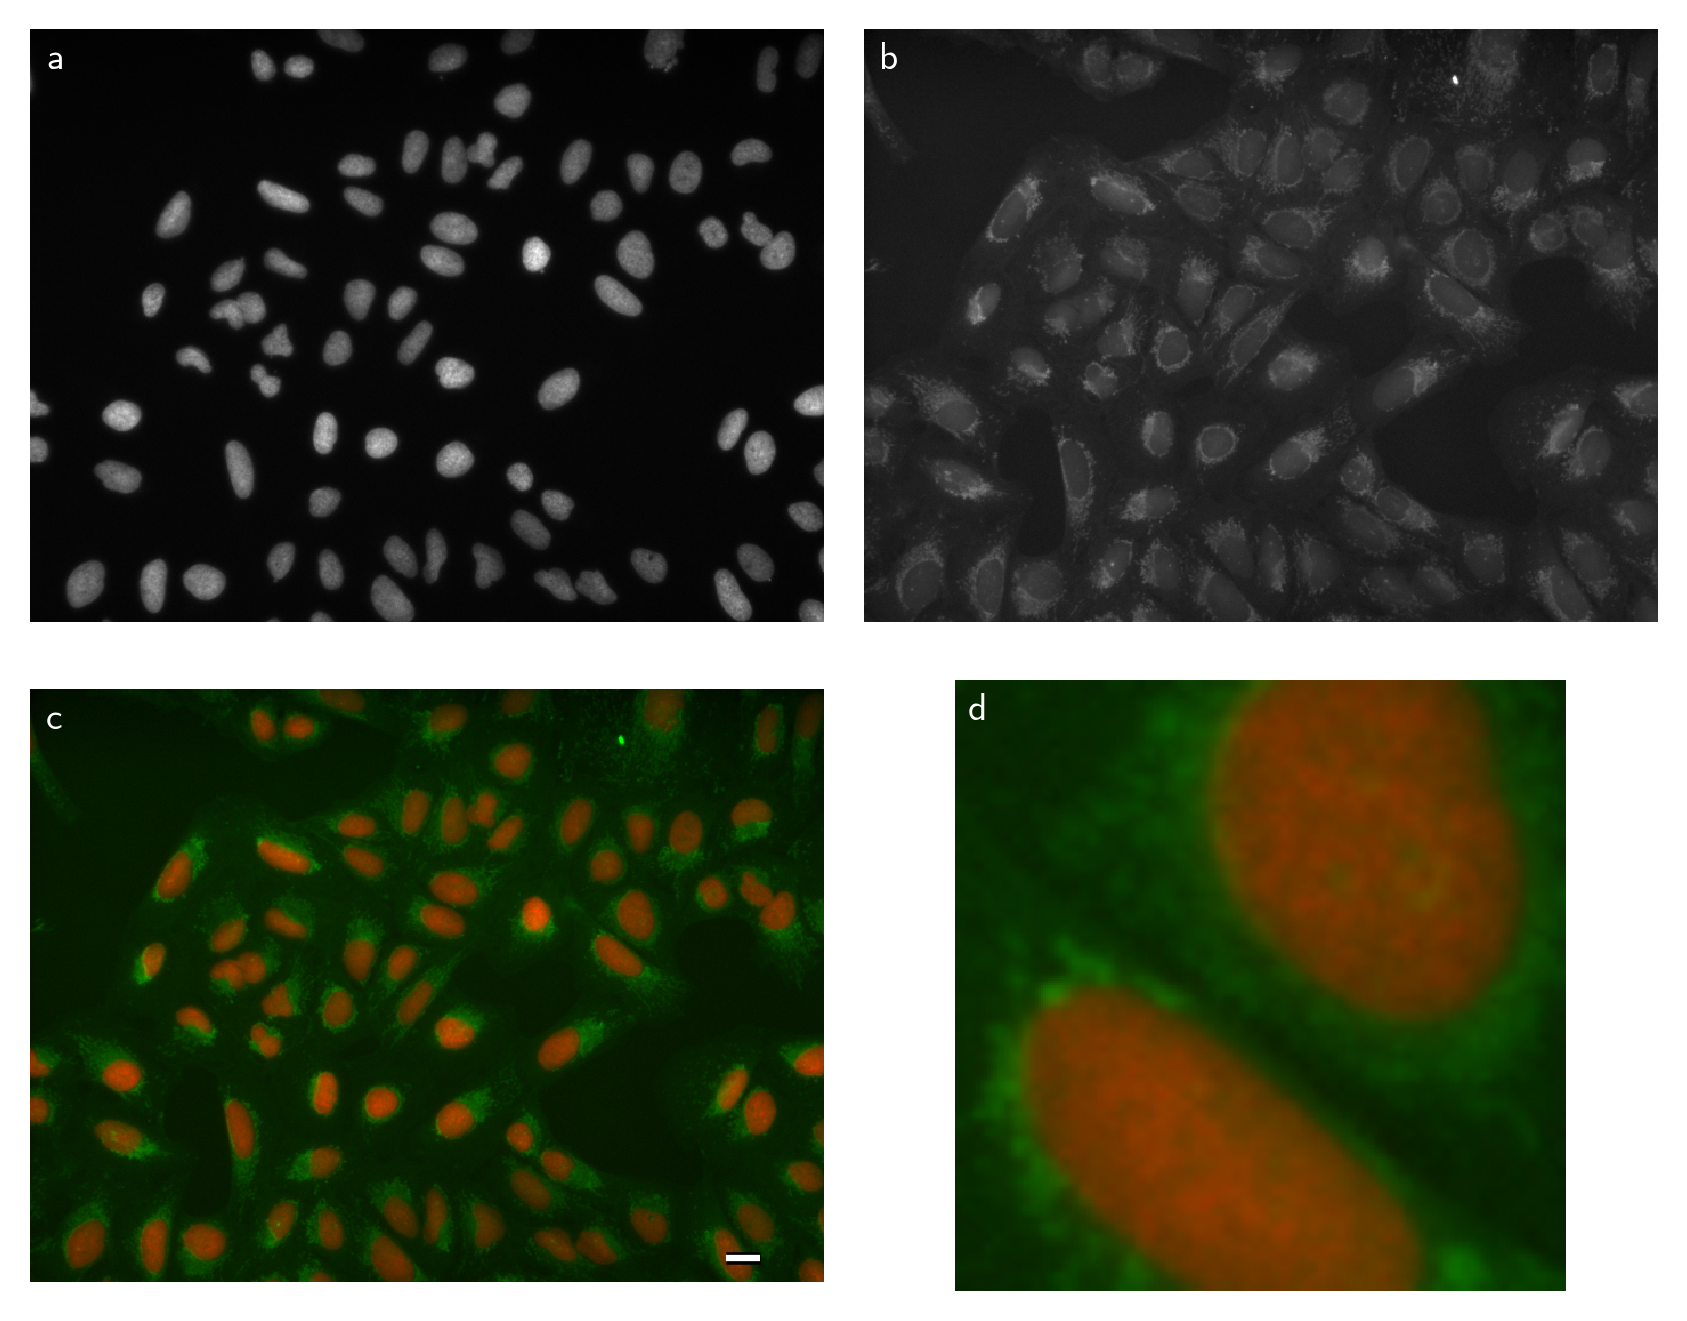
\includegraphics[width=\linewidth]{figures/ch08/ch08-08-case-v1-zh.png}};
  \begin{scope}[x={(img.south east)}, y={(img.north west)}]
    \node[chviiiissue] (m1) at (0.40, 0.92) {1};
    \node[chviiiissue] (m2) at (0.40, 0.45) {2};
    \node[chviiiissue] (m3) at (0.36, 0.09) {3};
    \draw[BookInk, line width=0.35pt] (0.372, 0.078) -- (0.424, 0.056);
    \node[chviiiissue] (m4) at (0.88, 0.12) {4};
    \node[chviiiissue] (m5) at (0.90, 0.92) {5};
  \end{scope}
  \node[chviiicap] (c1) at ([yshift=-1.8mm]img.south west)
    {\chviiimark{1}\enspace 各自自动对比度};
  \node[chviiicap] (c2) at ([yshift=-0.8mm]c1.south west)
    {\chviiimark{2}\enspace 红/绿};
  \node[chviiicap] (c3) at ([yshift=-0.8mm]c2.south west)
    {\chviiimark{3}\enspace 比例尺无依据};
  \node[chviiicap] (c4) at ([yshift=-0.8mm]c3.south west)
    {\chviiimark{4}\enspace 最亮细胞+双三次};
  \node[chviiicap] (c5) at ([yshift=-0.8mm]c4.south west)
    {\chviiimark{5}\enspace 未披露 $\gamma=0.6$};
\end{tikzpicture}
}
\caption{初稿中常见的五个问题（编号 1–5，见正文）。本图为按错误做法刻意生成的教学反例。终稿图注见案例小节。}\label{fig:ch08-08}\label{fig:ch08-08-v1}
\end{figure}

对照上述五处问题，列出逐条可核对的修改单：

\begin{Prompt}
修改单（v1 -> final）
1. 两个通道各用一套显示范围，所有面板共用：
   Hoechst 黑点 132、白点 1236（原始数值 p0.1 / p99.9）；
   MitoTracker 黑点 218、白点 1140（p0.1 / p99.9）。合成图使用同一组数值。
2. 取消伽马（gamma），全部为线性映射；处理记录写入“线性，无 gamma”。
3. 合成改为细胞核品红（R+B）、线粒体绿（G）；做一次红绿色盲模拟检查。
4. 比例尺按 0.656 µm/pixel 重算：50 µm = 76.2 px（a–c）；
   d 为 3× 最近邻放大，10 µm = 15.2 px × 3 = 45.7 px。
5. d 的选区改为一个核与线粒体信号都接近视野中位的细胞（坐标 (280, 328)–(344, 392)），
   在 c 上用 0.5 pt 白色方框标出；记录裁剪框像素坐标。
6. 放大用整数倍最近邻（3×），不使用双三次或任何“细节增强”。
7. 导出无损 PNG；保留原始 16 位 TIFF 与脚本、processing-log.json。
8. 在处理记录与图注中报告：线粒体通道有 12 个像素在采集时饱和（4095）。
\end{Prompt}

\textbf{第五步：在 \scidraw{} 组图工具排版、合并双层处理记录并完成终稿核验。}脚本按修改单生成四个 8 位无损 PNG 面板与 \path{processing-log.json} 后，进入 \scidraw{} 组图工具（\sdtool{multi-panel-figure-maker}）：导入四个面板，选择期刊双栏预设（Cell 或 Springer 双栏宽 $174\ \text{mm}$），设为 $2 \times 2$ 网格并自动编号 \textbf{a}--\textbf{d}（在组图工具内做的必要裁剪或旋转也会被自动记录），导出 ZIP 包（含 TIFF、PNG、PDF、PPTX 与组图处理记录），得到终稿（图~\ref{fig:ch08-09}）。

\begin{figure}[htbp]\centering
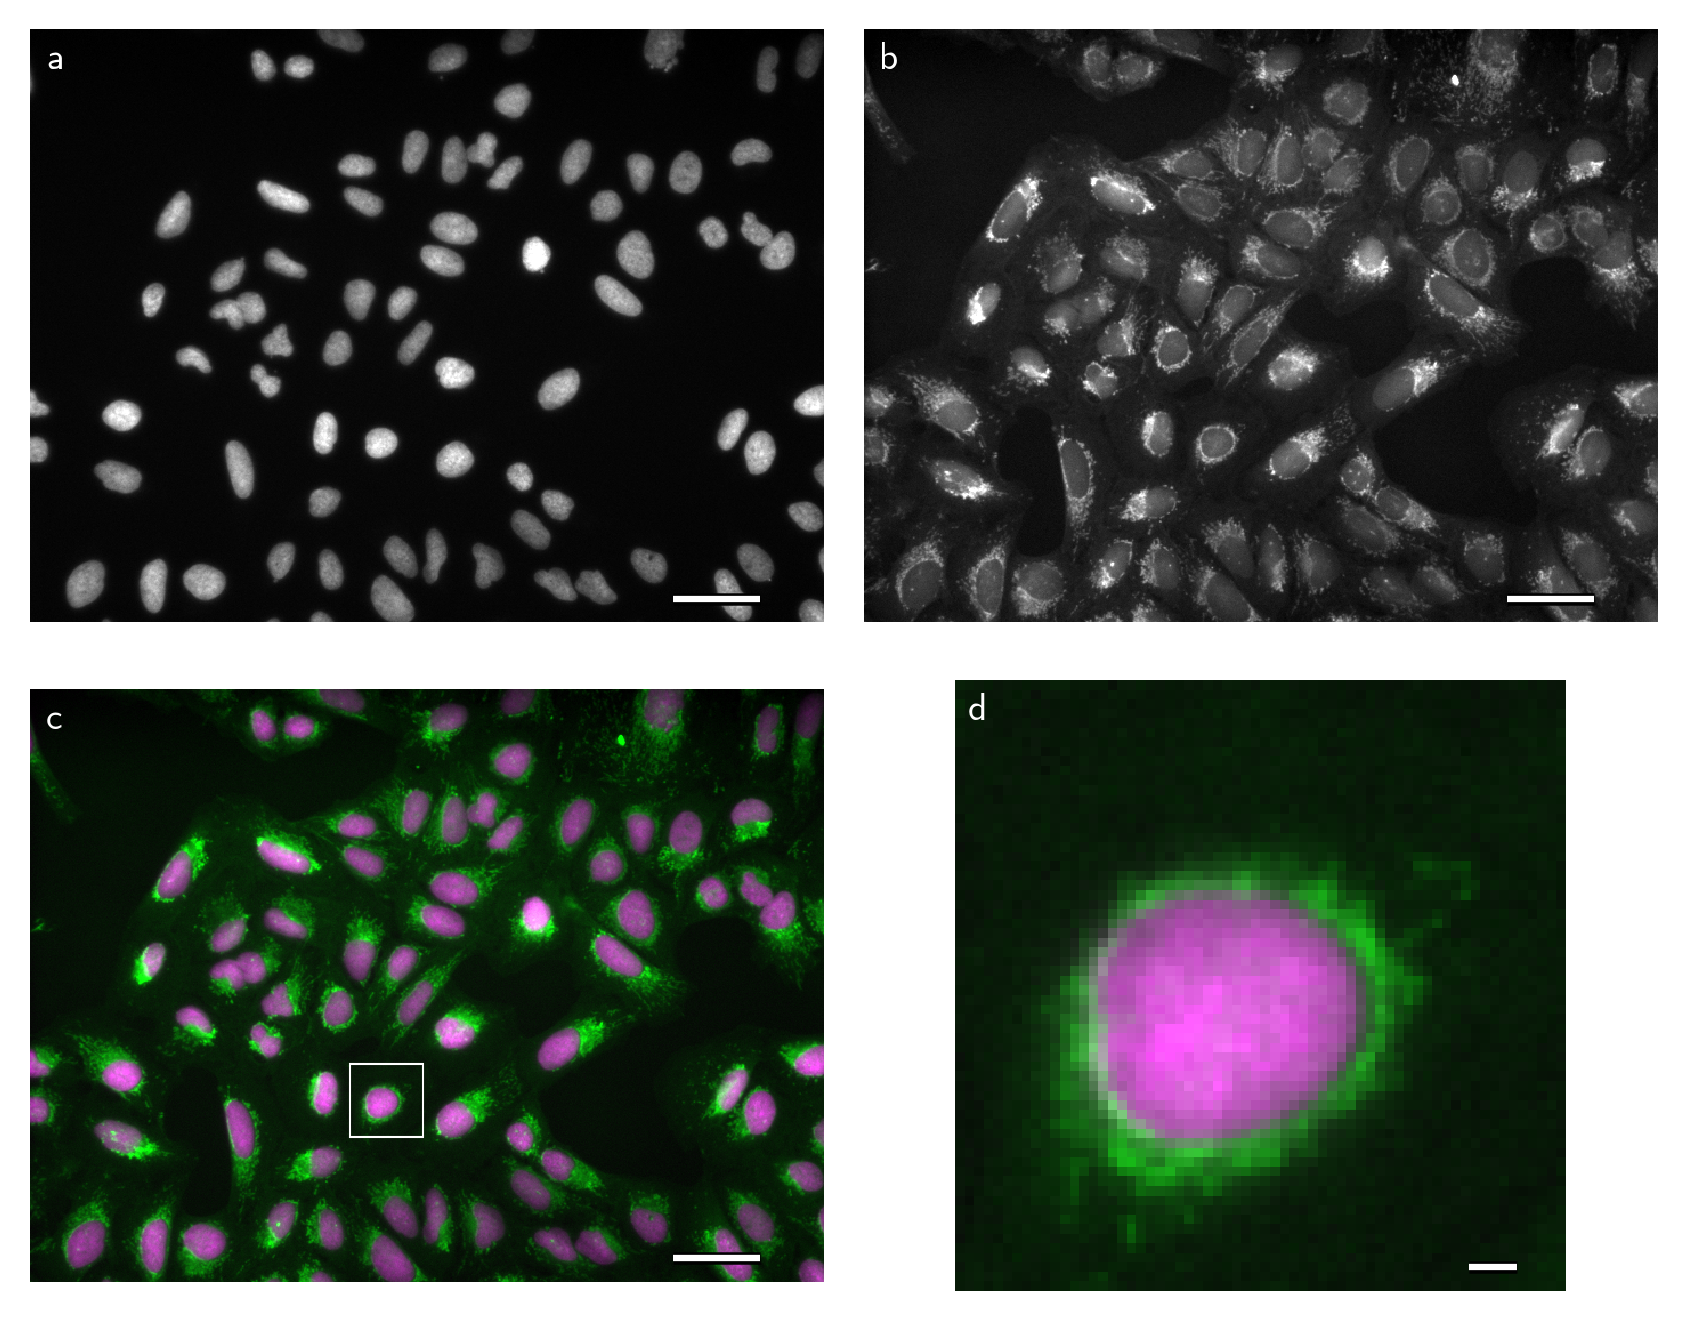
\includegraphics[width=0.88\linewidth]{figures/ch08/ch08-08-case-final-zh.png}
\caption{补充图 S1 | DMSO 对照条件下 U2OS 细胞的细胞核与线粒体染色。\textbf{a}，Hoechst 33342（细胞核）；\textbf{b}，MitoTracker Deep Red（线粒体）；\textbf{c}，合成图（细胞核品红，线粒体绿），白框为 d 的取样区域；\textbf{d}，c 中白框区域 3 倍最近邻放大。图像来自 BBBC022v1（板 20585，孔 A13，视野 1；CC0；Gustafsdottir 等，2013），$20\times$ 物镜，像素尺寸 $0.656\ \mu\text{m}$。所有面板为整图线性显示映射，无 $\gamma$ 或其他非线性调整；Hoechst 显示范围 $132\text{--}1236$、MitoTracker $218\text{--}1140$（原始 12 位数值），同一通道在各面板中设置相同。线粒体通道有 12 个像素在采集时达到饱和（$4095$），未做修补。比例尺：a--c 为 $50\ \mu\text{m}$，d 为 $10\ \mu\text{m}$。原始 16 位图像、处理脚本与处理记录见补充数据。}\label{fig:ch08-09}\label{fig:ch08-08-final}
\end{figure}

在这一步，作者必须特别注意两项平台边界与核验要点：
\begin{enumerate}
\item \textbf{合并上游处理记录与组图处理记录：}组图工具导出的处理记录会列出每个面板的原文件名、SHA-256、原始尺寸与位深、裁剪框、旋转/翻转、在图中的毫米尺寸、有效分辨率和重采样方式，并写明“除上述裁剪、旋转与缩放外，未对任何面板做亮度、对比度、颜色或内容改动”。必须明确：\textbf{这句声明只描述组图工具内部的操作。}由于导入的 PNG 面板已经在上游脚本中经过了显示范围映射与伪彩色合成，且组图工具当前不提供校准比例尺、通道标签与关联放大框功能（这些均在脚本中完成），导出 ZIP 也不包含原始 16 位 TIFF，作者必须把脚本生成的 \path{processing-log.json} 与组图处理记录\textbf{合并}成一份完整处理说明，否则读者会误以为面板未经任何显示调整。
\item \textbf{如实核查有效分辨率与补齐图注：}$696\ \text{px}$ 宽的原图在 $300\ \text{dpi}$ 下约为 $59\ \text{mm}$；在 $174\ \text{mm}$ 宽的 $2 \times 2$ 布局中每格约 $85\ \text{mm}$ 宽，此时有效分辨率约为 $208\ \text{dpi}$。对此，作者要么接受较低的有效分辨率并在说明中如实写出原始像素尺寸，要么缩小面板物理尺寸以达到 $300\ \text{dpi}$，\textbf{绝不能用插值放大冒充分辨率}。随后用图片检查工具（\sdtool{figure-checker}）检查导出图的格式、分辨率、灰度与色觉风险（注意它只做技术检查，不代表科学审核）；再用图注辅助工具（\sdtool{figure-legend}）起草“看图可见”的描述，由作者亲手补齐染料、像素尺寸、显示范围、饱和说明与比例尺长度（工具按设计不编造放大倍数、比例尺或方法）。终稿对应的英文图注与交付核验表如下：
\end{enumerate}

\begin{Prompt}
Supplementary Fig. S1 | Nuclear and mitochondrial staining of U2OS cells under DMSO control
conditions. a, Hoechst 33342 (nuclei). b, MitoTracker Deep Red (mitochondria). c, Merge
(nuclei magenta, mitochondria green); the white box marks the region shown in d. d, The
boxed region in c enlarged 3× with nearest-neighbour sampling. Images are from BBBC022v1
(plate 20585, well A13, site 1; CC0; Gustafsdottir et al., 2013), acquired with a 20×
objective at 0.656 µm per pixel. All panels use whole-image linear display mapping with no
gamma or other non-linear adjustment; display ranges were 132–1236 (Hoechst) and 218–1140
(MitoTracker) in raw 12-bit values and are identical for each channel across panels. Twelve
pixels in the mitochondrial channel were saturated at acquisition (4095) and were not
altered. Scale bars, 50 µm (a–c) and 10 µm (d). Raw 16-bit images, the processing script
and the processing log are provided as Supplementary Data.
\end{Prompt}

\begin{table}[htbp]\centering\footnotesize
\setlength{\tabcolsep}{3pt}
\renewcommand{\arraystretch}{1.15}
\caption{主案例终稿（补充图 S1）核验表。}\label{tab:ch08-verify}
\begin{tabularx}{\linewidth}{@{}>{\raggedright\arraybackslash}p{25mm}YY@{}}
\toprule
\textbf{核验项} & \textbf{核验方法} & \textbf{实测结果} \\
\midrule
输入文件哈希 & 脚本断言四个面板的输入 SHA-256 与原图目录一致 & 与表~\ref{tab:ch08-catalog} 及目录 CSV 完全一致，原件未改动 \\
显示范围与线性 & 对照 \path{processing-log.json} 与图注数值 & Hoechst $132\text{--}1236$、MitoTracker $218\text{--}1140$，全图线性无 $\gamma$，12 个饱和像素已报告 \\
比例尺像素数 & 按 $0.656\ \mu\text{m/px}$ 复算并在导出图上量取 & a--c 的 $50\ \mu\text{m} = 76.2\ \text{px}$；d（$3\times$）的 $10\ \mu\text{m} = 45.7\ \text{px}$，吻合 \\
放大框与裁剪框 & 核对 c 上白框坐标与 d 的裁剪坐标 & 同一组中位细胞坐标 $(280, 328)\text{--}(344, 392)$，$3\times$ 最近邻采样 \\
色觉与记录合并 & Machado（2009）模拟与 \sdtool{figure-checker}；检查双层记录 & 红绿色盲模拟下品红/绿可区分；已合并上游显示映射记录与组图裁剪/缩放记录 \\
\bottomrule
\end{tabularx}
\end{table}

\section{AI 在实验图像呈现中能做什么与不能做什么}

实验图像呈现各环节中 AI 与作者的职责边界汇总于表~\ref{tab:ch08-01}。

\begin{table}[htbp]\centering\footnotesize
\setlength{\tabcolsep}{3pt}
\renewcommand{\arraystretch}{1.15}
\caption{实验图像呈现各环节中 AI 能做什么、不能做什么与作者必须核对的内容。}\label{tab:ch08-01}
\begin{tabularx}{\linewidth}{@{}>{\raggedright\arraybackslash}p{18mm}YYY@{}}
\toprule
\textbf{环节} & \textbf{AI 能做} & \textbf{AI 不能做} & \textbf{作者要核对} \\
\midrule
原图整理 & 起草原图目录模板；写读取元数据、计算哈希的脚本 & 判断哪个文件是“原始”的；补写缺失的采集参数 & 原件只读；哈希与目录一致；采集参数有出处 \\
呈现计划 & 按面板目的列出每步处理与需要披露的内容；区分线性与非线性操作 & 决定哪个视野“有代表性”；判断生物学含义 & 选区依据、对照是否齐全、计划是否满足期刊规则 \\
显示映射 & 写按分位数设置黑白点、统一应用于各面板并输出参数的脚本 & 自动“调到好看”；对局部区域单独调整 & 各面板参数一致；无数据被截断；非线性调整已披露 \\
伪彩色 & 推荐色盲友好组合；写色觉模拟脚本；\sdtool{figure-checker} 做色觉风险检查 & 保证所有读者都能区分；替代分通道灰度 & 品红/绿或分通道；模拟检查结果；图注写明颜色对应 \\
裁剪与放大 & 写记录裁剪框和放大倍数的脚本；组图工具记录裁剪、旋转、缩放与有效分辨率 & 补出原图中没有的细节；“超分辨率”证据图 & 选区不偏倚；放大用最近邻或声明插值；有效分辨率够用 \\
比例尺 & 按像素尺寸计算比例尺长度 & 在没有校准信息时“估计”像素尺寸；从图像内容推断尺度 & 像素尺寸来源（元数据/数据条/标定）；放大后重算 \\
增强与修复 & 无——证据图像路径上不使用生成式模型 & 去噪、锐化、补全、去伪影、“变清晰” & 全流程无生成式操作；确定性处理（如反卷积）的方法与参数已写明 \\
图注与方法 & \sdtool{figure-legend} 起草可见内容描述；助手据处理记录起草方法段 & 编造染料、物镜、像素尺寸、样本量 & 来源、许可、显示设置、饱和说明、比例尺长度齐全 \\
\bottomrule
\end{tabularx}
\end{table}

\section{本章检查清单}

\begin{itemize}
\item 原件只读保存，目录中有文件名、来源、位深、尺寸、像素尺寸、SHA-256、许可。
\item 所有显示调整都是整图施加；同一比较中的面板使用相同显示设置，参数已记录。
\item 没有让数据消失的截断；饱和像素已报告。
\item $\gamma$、曲线等非线性调整（若有）已在图注中披露。
\item 多通道合成使用色盲友好配色或提供分通道灰度；做过色觉模拟。
\item 裁剪选区有书面依据；放大框在原图中标出；放大倍数与插值方式已写明。
\item 比例尺长度可由像素尺寸复算；没有校准信息时不画比例尺，并在图注说明。
\item 不同视野、时间或样品的图像没有被拼成“同一视野”；必要的并列有清晰分隔并在图注说明。
\item 证据图像的任何像素都没有经过生成式 AI 处理。
\item 组图工具的处理记录与上游处理说明已合并；原始文件与脚本另存并随补充数据提供。
\end{itemize}

\section{练习}

\begin{enumerate}
\item \textbf{（判断题组，纸笔）}针对下列 6 条处理描述：(1)“对处理组单独提高亮度以便看清”；(2)“对整幅合成图统一施加 $\gamma = 0.8$ 并在图注说明”；(3)“用克隆工具去掉一粒灰尘”；(4)“把两个视野的细胞拼到同一面板且不加分隔线”；(5)“按 $0.1\%/99.9\%$ 分位数设置线性范围并统一应用于所有面板”；(6)“把 JPEG 截图交给 AI 放大到 4K”。逐条判断属于“可接受”“可接受但须披露”还是“不可接受”，并引用第 5 节的规则说明理由（参考答案见附录）。
\item \textbf{（比例尺计算，脚本）}下载 \path{Leaf_epidermis.jpg}（Wikimedia Commons），自己编写脚本测量底部数据条中标尺线的像素长度，计算像素尺寸；为一个 $600 \times 600\ \text{px}$ 的裁剪区域画 $100\ \mu\text{m}$ 比例尺；再把该区域 $2\times$ 最近邻放大并重算比例尺。与本章数值（$720\ \text{px}$、$0.278\ \mu\text{m/px}$）比较，并说明这个像素尺寸依赖什么前提。
\item \textbf{（\scidraw{} 实操）}用本章脚本生成的四个终稿面板，在科研绘图向导（\sdtool{figure-workflow}）中选择“已有图片组图”路线，进入组图工具（\sdtool{multi-panel-figure-maker}）：选 $174\ \text{mm}$ 双栏预设、$2 \times 2$ 网格、自动编号；导出 ZIP；打开处理记录，找出“未做亮度、对比度、颜色改动”的声明，写一段话说明为什么这句话对本图不完整，并把脚本的 \path{processing-log.json} 合并成一份完整处理说明。最后用 \sdtool{figure-checker} 检查导出图，记录它报告了什么、没有报告什么。
\end{enumerate}

\section*{参考文献}

\begin{itemize}
\item Bik EM, Casadevall A, Fang FC. The prevalence of inappropriate image duplication in biomedical research publications. \textit{mBio}. 2016;7(3):e00809-16. doi:10.1128/mBio.00809-16
\item Crameri F, Shephard GE, Heron PJ. The misuse of colour in science communication. \textit{Nature Communications}. 2020;11:5444. doi:10.1038/s41467-020-19160-7
\item Cromey DW. Avoiding twisted pixels: ethical guidelines for the appropriate use and manipulation of scientific digital images. \textit{Science and Engineering Ethics}. 2010;16(4):639--667. doi:10.1007/s11948-010-9201-y
\item Gustafsdottir SM, Ljosa V, Sokolnicki KL, et al. Multiplex cytological profiling assay to measure diverse cellular states. \textit{PLoS ONE}. 2013;8(12):e80999. doi:10.1371/journal.pone.0080999
\item Jambor H, Antonietti A, Alicea B, et al. Creating clear and informative image-based figures for scientific publications. \textit{PLOS Biology}. 2021;19(3):e3001161. doi:10.1371/journal.pbio.3001161
\item Ljosa V, Sokolnicki KL, Carpenter AE. Annotated high-throughput microscopy image sets for validation. \textit{Nature Methods}. 2012;9(7):637. doi:10.1038/nmeth.2083
\item Machado GM, Oliveira MM, Fernandes LAF. A physiologically-based model for simulation of color vision deficiency. \textit{IEEE Transactions on Visualization and Computer Graphics}. 2009;15(6):1291--1298. doi:10.1109/TVCG.2009.113
\item Rossner M, Yamada KM. What's in a picture? The temptation of image manipulation. \textit{Journal of Cell Biology}. 2004;166(1):11--15. doi:10.1083/jcb.200406019
\item Schmied C, Jambor HK. Effective image visualization for publications -- a workflow using open access tools and concepts. \textit{F1000Research}. 2020;9:1373. doi:10.12688/f1000research.27140.1
\item Wong B. Points of view: Color blindness. \textit{Nature Methods}. 2011;8(6):441. doi:10.1038/nmeth.1618
\item Broad Bioimage Benchmark Collection. BBBC022v1 image set (U2OS Cell Painting). \url{https://bbbc.broadinstitute.org/BBBC022} (accessed 2026-10-29).
\item Nature Portfolio. Editorial policies: Image integrity and standards. \url{https://www.nature.com/nature-portfolio/editorial-policies/image-integrity} (accessed 2026-10-29).
\item Nature Portfolio / Springer Nature. Editorial policies: Artificial Intelligence (AI). \url{https://www.nature.com/nature-portfolio/editorial-policies/ai} (accessed 2026-10-29).
\item Okabe M, Ito K. Color Universal Design (CUD): How to make figures and presentations that are friendly to colorblind people. \url{https://jfly.uni-koeln.de/color/} (accessed 2026-10-29).
\end{itemize}
